\documentclass[fleqn,10pt]{wlscirep}
\usepackage[utf8]{inputenc}
\usepackage[T1]{fontenc}
\usepackage{graphicx}
\usepackage{booktabs}
\usepackage{amsmath,amsfonts,amsthm}
\usepackage{array}
\usepackage{xr}
\externaldocument{supplementary}

\renewcommand{\topfraction}{0.9}\renewcommand{\bottomfraction}{0.8}\renewcommand{\textfraction}{0.07}\renewcommand{\floatpagefraction}{0.75}
\setcounter{topnumber}{4}\setcounter{bottomnumber}{3}\setcounter{totalnumber}{8}

\newtheorem{lemma}{Lemma}
\newtheorem{theorem}{Theorem}
\newtheorem{corollary}{Corollary}

\begin{document}

\title{FanarVSE: Fast, Memory-Light GPU Vector Search with Error Bars from Coding Theory}

%======================================================================
%==============================AUTHORS=================================
%======================================================================
\author[1,*]{Mohammed Mohsen}
\affil[1]{Information Systems Department, Faculty of Computers and Artificial Intelligence, Fayoum University, Fayoum, Egypt}
\affil[*]{Corresponding author: Mohammed Mohsen (mm5987@fayoum.edu.eg)}

%======================================================================
%==============================Abstract================================
%======================================================================
\begin{abstract}
GPU vector search is limited by memory: graph indexes keep full-precision vectors on the device, and compressed indexes lose recall. We show that three results from coding theory turn this into a design. First, the unbiased RaBitQ estimator holds for any codebook after a random rotation, with an exact, data-independent error law whose variance depends on the codebook only through one number; the best codebook is the best spherical code, and predicted and measured errors agree. Second, bitshift trellis codes, decodable on tensor cores, come within 0.24\,dB of the Shannon bound, and an identification-rate argument suggests how small the first-stage filter can be. Third, the error law gives error bars that leave about six full-precision reads per query, or 18 with a per-query failure bound of 0.5\%, so full vectors can stay in host RAM or on an NVMe drive. An exact threshold selection, a first stage coded relative to each cell's mean, a batch path without host synchronisation and a tiered refinement code whose error bars follow from the same law make the system fast as well as small. On one million OpenAI embeddings and a 6\,GB laptop GPU, our system, FanarVSE, reaches recall@10 0.992 at 22{,}649 queries per second with 570 bytes of GPU memory per vector, shared tables included: 5.1$\times$ the throughput of CAGRA and 2.8--3.0$\times$ that of IVF-RaBitQ at the same recall, with 5.6$\times$ and 3.2$\times$ less memory, and the index builds in 28\,s. It is the fastest of the three at every recall we measured from 0.95 to 0.998 and reaches 0.999 at 7.5$\times$ the throughput of exact fp16 search, where neither CAGRA nor IVF-RaBitQ goes beyond 0.998. For large batches, an optional throughput mode with int8 first-stage codes and a refinement code scored by lookup tables (787 bytes per vector) reaches 0.9905 at 83{,}606 queries per second in batches of 2{,}000 and at 90{,}391 in batches of 16{,}000, 19--20$\times$ the throughput of CAGRA, which does not grow with the batch, and 0.996 at 54{,}664 (24$\times$). With 100 neighbours it is 2.5$\times$ faster than CAGRA at recall 0.99, and a single query takes 0.63\,ms at recall 0.991, 1.2$\times$ faster than CAGRA. With every per-vector array in host RAM, read by the GPU over PCIe, FanarVSE keeps 7.7\,MB on the GPU for a million vectors, under eight bytes per vector, and still reaches 0.991 at 13{,}841 queries per second: 3.1$\times$ the throughput of CAGRA and 1.7--1.9$\times$ that of IVF-RaBitQ, with 415$\times$ and 240$\times$ less GPU memory. With 66 bytes per vector on the GPU and full vectors on an NVMe drive it reaches 0.992 at 9{,}057 queries per second. On five more sets, among them 1.28 million SigLIP and 258k DINOv2 image embeddings and 2.25 million arXiv text embeddings, it is the fastest index above recall 0.98--0.995; below, IVF-RaBitQ (on the image sets) and CAGRA (on the largest set) are faster.
\end{abstract}
\maketitle

\section{Introduction}
Embedding search is now a default component of retrieval-augmented generation, recommendation and deduplication. On GPUs, the fastest indexes are graphs (CAGRA~\cite{ootomo2024cagra}) and brute-force or inverted-file scans (FAISS~\cite{douze2024faiss}, cuVS). The first group is fast but keeps the dataset in device memory: one million 1536-dimensional OpenAI embeddings occupy 3.1\,GB in fp16, half of a 6\,GB card. The second group compresses vectors with product quantization (PQ)~\cite{jegou2011pq} and pays for it in recall.

Recent work on CPUs has shown that randomly rotated scalar codes with an unbiased estimator (RaBitQ~\cite{gao2024rabitq,gao2025extended}, TurboQuant~\cite{zandieh2025turboquant}) are far better than PQ at ranking. This paper asks how far that line can be pushed when the target is \emph{GPU memory per vector} at high recall, and answers with three pieces of theory, each of which became a component of a working system.

\paragraph{Contributions.} The first contribution is a \textbf{codebook-agnostic unbiasedness theorem} (\S\ref{sec:theory}). The RaBitQ estimator $\langle q,\bar o\rangle/c$ is unbiased for any deterministic quantizer applied after a Haar rotation, with variance $\|q_\perp\|^2(1-c^2)/(c^2(d-1))$ and an exact standardised error law. The best codebook is the best spherical code; lattice codes (E8, BW16) and trellis codes beat the hypercube, in the order the formula predicts, on four embedding models (and the order breaks, as the theory says it may, on sparse data without the rotation). We test the theorem and the law directly: per query--vector pair over 1{,}000 rotations, conditionally on $c$ and on the candidate's rank, and down to eight dimensions, where the exact law and a Gaussian differ (\S\ref{sec:tests}).

Second, we bring \textbf{near-Shannon trellis codes to vector search} (\S\ref{sec:trellis}). Bitshift trellis codes, borrowed from LLM weight quantization (QTIP~\cite{tseng2024qtip}, after TCQ~\cite{marcellin1990tcq}), lower Gaussian distortion from 1.64\,dB to 0.24\,dB above the Shannon bound at 1 bit per coordinate and raise estimator recall from 0.828 to 0.855 at the same size. A window property lets a Triton kernel decode them in registers and feed tensor cores directly.

Third, we \textbf{size the filter stage by the identification rate} (\S\ref{sec:ident}). The first stage only needs to \emph{identify} candidates, not reconstruct vectors. The identification rate~\cite{ingber2015identification}, with an explicit derivation and its sensitivity to the effective dimension, suggests about 140 bits per vector on our data; a 202-bit trellis code keeps 98.9\% of the true top-10 within 200 candidates. Out of sample it is right to within a factor of two, but it does not account for the candidate budget.

Fourth, we use the theorem for \textbf{error-bar refinement with a coverage guarantee} (\S\ref{sec:system}). The exact error law classifies candidates as surely in, surely out or ambiguous. We prove that if every interval covers its true score, the result equals the exact top-$k$ of the candidate set, which turns the error law into a per-query failure bound. Only ambiguous candidates are read in full precision: 5.7--5.9 reads per query. This matches the recall of a full exact rerank with 35$\times$ fewer reads and 2.9$\times$ the throughput, and makes an NVMe tier for full vectors practical.

Fifth, the system adds \textbf{an exact threshold selection, a cell-residual first stage and tiered refinement} (\S\ref{sec:system}). Stage 1 sets a threshold from a few nearby cells, emits only items above it in one pass that decodes each code block once, and verifies by counting that the result is the exact top $K$. It codes each vector relative to its cell's mean, with the per-(query, cell) constant read from the sorted work list, which halves the candidates needed on clustered image embeddings, and a fixed-size work list makes the whole batched search one CUDA graph. The refinement code allocates bits across principal directions in tiers, each of which satisfies Theorem~\ref{thm:main}, so the error bars carry over with a sub-Gaussian tail bound. Together with 4{,}096 cells and exact reads from host memory by zero-copy, they raise throughput 3.7$\times$ (and recall from 0.992 to 0.996) at the same probes and cut GPU memory from 820 to 570\,B/vector (shared tables included).

Sixth, we evaluate \textbf{FanarVSE on the same GPU} as its baselines (\S\ref{sec:eval}): against CAGRA, cuVS IVF-RaBitQ, FAISS-GPU and cuVS IVF-PQ on eight datasets (three text-embedding models, GloVe, and SigLIP and DINOv2 image embeddings, up to 2.25M vectors), with $k=10$ and $k=100$, batch sizes from 1 to 16{,}000, five random seeds, five rotation types, and both operating systems, including variants with 66\,B and with under 8\,B of GPU memory per vector, and a throughput mode (int8 stage 1, stage 2 by lookup tables, 787\,B per vector) that serves 19--27$\times$ CAGRA's queries per second from recall 0.99 to 0.997 at batches of 2{,}000 to 16{,}000.

Finally, we \textbf{document negative results} (\S\ref{sec:negative}), including the \emph{error-isotropy principle}: decoders that minimise mean squared error (MSE), such as the Bussgang linear MMSE decoder, cut the reconstruction error by up to two thirds and still lower recall, because their error concentrates in the directions that queries share; we measure this concentration directly in the error covariance and confirm the mechanism with synthetic errors of controlled covariance.

We do not claim the second-stage refinement code: rotation plus a per-coordinate Lloyd--Max quantizer plus a per-vector correction is TurboQuant~\cite{zandieh2025turboquant}, implemented on CPU by turbovec~\cite{turbovec}. Bit allocation across dimensions is also prior art~\cite{saq2025,monavec2026,beyonduniform2026}.

\section{Background and Related Work}\label{sec:related}
\paragraph{Graph indexes.} HNSW~\cite{malkov2020hnsw} dominates CPU search; CAGRA~\cite{ootomo2024cagra} adapts graph search to GPUs with high throughput. Both read full or lightly compressed vectors during traversal, so device memory grows with the raw dataset.

\paragraph{Quantization for search.} PQ~\cite{jegou2011pq} learns sub-codebooks by k-means and scores with lookup tables. LVQ and LeanVec~\cite{aguerrebere2023lvq,tepper2023leanvec} combine per-vector scalar quantization with dimensionality reduction. RaBitQ~\cite{gao2024rabitq} randomly rotates a normalised residual, keeps the sign bits and stores $c=\langle o,\bar o\rangle$, which gives an unbiased inner-product estimator with an error bound; extended RaBitQ~\cite{gao2025extended} generalises it to more bits. TurboQuant~\cite{zandieh2025turboquant} uses a rotation and a Lloyd--Max scalar codebook. SAQ~\cite{saq2025} and others~\cite{monavec2026,beyonduniform2026} allocate bits unequally across dimensions. BlockQuant~\cite{ann2026blockquant} quantizes blocks of two or three Haar-rotated coordinates with a codebook derived from the spherical marginal, and rescales by $1/\langle z,\bar z\rangle$ for an unbiased inner product; it is an instance of Theorem~\ref{thm:main}, and its gains over coordinate-wise codes match our design rule that a better spherical code (larger $c$) gives a smaller estimator variance. MRQ~\cite{yang2024mrq} projects vectors onto their leading principal subspace, codes that subspace with RaBitQ and summarises the tail by its variance; on CPUs it decides which candidates to re-rank with RaBitQ's concentration bound for the coded part and Chebyshev's inequality for the tail. FanarVSE's stage 1 uses the same projection, but on our data the truncated tail is neither isotropic nor unbiased (on stage-1 candidates its variance is 6$\times$ that of an isotropic model and it shifts the standardised error by $+0.25$), so we use stage 1 only to select candidates and place error bars on a code of the full residual, whose error law is exact; a Chebyshev-type interval would cost about 40 instead of 6 reads per query (Table~\ref{tab:z}).

\paragraph{High-recall GPU and tiered search.} IVF-RaBitQ for GPUs~\cite{shi2026ivfrabitq}, now part of cuVS, combines an inverted file with RaBitQ and its multi-bit extension in fused kernels and reports higher throughput than CAGRA at recall 0.95 with much faster builds; it ranks by the estimator and reads no full vectors. It is the closest system to ours and we compare with it directly (\S\ref{sec:eval}). Lychee~\cite{zhao2026lychee} screens the probed inverted lists on tensor cores with anchor-based bounds and certifies that its result equals that of IVF-Flat over the same lists, reading a few hundred full vectors per query. PilotANN~\cite{gui2026pilotann} keeps a sampled subgraph with reduced vectors on the GPU and refines on the CPU, and FaTRQ~\cite{zhang2026fatrq} refines coarse distances with ternary residuals streamed from far memory and stops early once a candidate is clearly out of the top-$k$. RSLM~\cite{lenhardt2026rslm} uses rotated, scaled Lloyd--Max scalar codes of 1--4 bits per dimension, with a block-wise cascaded Walsh--Hadamard rotation, for both scoring and rescoring on CPUs; its codec is close to our stage 2.

\paragraph{Codes from communication theory.} Lattices such as E8 and the Barnes--Wall lattice BW16~\cite{conway1999sphere} are classical dense packings. Trellis-coded quantization~\cite{marcellin1990tcq} reaches close to the rate--distortion bound for memoryless sources; QTIP~\cite{tseng2024qtip} introduced the \emph{bitshift} trellis, whose states are overlapping bit windows, for parallel decoding of LLM weights. Identification via channels~\cite{ahlswede1989identification} and its source-coding counterpart for similarity queries~\cite{ingber2015identification} quantify how many bits are needed to answer ``is $x$ similar to $q$?'' rather than to reproduce $x$.

\section{Theory}\label{sec:theory}
\subsection{Setting}
Let $o\in S^{d-1}$ be a unit residual (a data vector minus its cell centroid, normalised), $P$ a Haar-random orthogonal matrix, and $C:\mathbb{R}^d\to\mathbb{R}^d\setminus\{0\}$ any deterministic quantizer (hypercube, lattice, trellis). The code is
\[
\bar o=\frac{P^\top C(Po)}{\|C(Po)\|},\qquad c=\langle o,\bar o\rangle,
\]
where $c$ is stored per vector, and the estimator is $\widehat{\langle q,o\rangle}=\langle q,\bar o\rangle/c$.

\begin{lemma}[Invariance]\label{lem:inv}
For every rotation $R$ with $Ro=o$, the pairs $(c,\bar o)$ and $(c,R\bar o)$ have the same distribution.
\end{lemma}
\begin{proof}
Let $P'=PR^\top$. $P'$ is Haar-distributed by right invariance, and $P'o=PR^\top o=Po$. Hence $C(P'o)=C(Po)$ and the code built from $P'$ is $R\bar o$. Since $P'$ and $P$ have the same law, so do $(c,\bar o)$ and $(c,R\bar o)$; $c$ is unchanged because $\langle o,R\bar o\rangle=\langle R^\top o,\bar o\rangle=\langle o,\bar o\rangle$.
\end{proof}

\begin{theorem}[Codebook-agnostic unbiasedness]\label{thm:main}
Write $\bar o=c\,o+e$ with $e\perp o$. Conditional on $c$, $e$ is uniform on the sphere of radius $\sqrt{1-c^2}$ in $o^\perp$. Consequently
\[
\mathbb{E}\!\left[\tfrac{\langle q,\bar o\rangle}{c}\,\middle|\,c\right]=\langle q,o\rangle,\qquad
\mathrm{Var}\!\left[\tfrac{\langle q,\bar o\rangle}{c}\,\middle|\,c\right]=\frac{\|q_\perp\|^2(1-c^2)}{c^2(d-1)},
\]
where $q_\perp$ is the component of $q$ orthogonal to $o$.
\end{theorem}
\begin{proof}
By Lemma~\ref{lem:inv} the conditional law of $e$ is invariant under all rotations of $o^\perp$; the only such law with a fixed norm is the uniform law on that sphere. Its mean is zero and $\mathbb{E}\langle q,e\rangle^2=\|q_\perp\|^2\|e\|^2/(d-1)$.
\end{proof}

The theorem gives more than a variance. Write $\sigma=\|q_\perp\|\sqrt{1-c^2}/(c\sqrt{d-1})$ and $Z=(\widehat{\langle q,o\rangle}-\langle q,o\rangle)/\sigma$.
\begin{corollary}[Exact error law]\label{cor:law}
Conditional on $c$, $Z\stackrel{d}{=}\sqrt{m}\,u_1$ with $m=d-1$ and $u$ uniform on $S^{m-1}$; equivalently $Z^2/m\sim\mathrm{Beta}(\tfrac12,\tfrac{m-1}{2})$. Hence $\mathbb{E}Z=0$, $\mathbb{E}Z^2=1$, the excess kurtosis is $-6/(m+2)$, $P(|Z|>z)=I_{1-z^2/m}\!\left(\tfrac{m-1}{2},\tfrac12\right)$, and $P(|Z|>z)\le 2e^{-z^2/2}$. The law does not depend on the data, the query or the codebook.
\end{corollary}
\begin{proof}
$\langle q,e\rangle/\|e\|=\|q_\perp\|\langle \hat q_\perp,u\rangle$ with $u=e/\|e\|$ uniform on the unit sphere of $o^\perp$ (dimension $m$), and $\langle \hat q_\perp,u\rangle$ has the law of one coordinate of $u$. The moments and the Beta form are standard; the tail bound is the usual concentration of a sphere coordinate.
\end{proof}
For $d=1536$ the law is Gaussian to three decimals: the excess kurtosis is $-0.004$ and $P(|Z|>2)$, $P(|Z|>3)$ are 4.546\% and 0.267\% (Gaussian: 4.550\%, 0.270\%). Concentration then gives an error bound of order $\sqrt{(1-c^2)/c^2}\,\|q_\perp\|/\sqrt d$, which is RaBitQ's bound with its constant $c\approx\sqrt{2/\pi}$ replaced by the codebook's $c$. In low dimensions the law is far from Gaussian (at $d=8$, $P(|Z|>2)=3.0\%$ and $P(|Z|>3)=0$); Section~\ref{sec:tests} uses this to test the corollary directly.

\paragraph{Structured rotations.} The theorem needs a Haar rotation; fast systems use structured ones such as random signs plus Walsh--Hadamard transforms~\cite{lenhardt2026rslm}. Under one or three rounds of signs plus a block Walsh--Hadamard transform, or block-diagonal Haar rotations with blocks of 64 or even 8 coordinates, the standardised error of FanarVSE's stage-2 code, its recall and its reads are indistinguishable from those under a dense Haar rotation; only removing the rotation biases the error (Supplementary Table~\ref{tab:rot}). The guarantees below therefore hold as stated for Haar rotations and, empirically, for these structured rotations.

\begin{corollary}[Design rule]
At a fixed bit budget, the codebook that minimises estimator variance is the one with the largest typical $c$, that is, the best spherical code on rotated, near-Gaussian blocks. The relative estimator error is $\sqrt{1-c^2}/c$.
\end{corollary}

\paragraph{Validation.} Table~\ref{tab:c} lists $c$ for several codebooks at 1 bit per dimension on 20k rotated OpenAI-1536 vectors. Replacing RaBitQ's hypercube by per-8-block E8 shell codewords changes $c$ from 0.798 to 0.826; the corollary predicts a 9.4\% smaller estimator standard deviation and we measure 9.5\%. Inside an IVF index with identical cells, rotation, per-vector factors and bytes, the lattice codebooks raise recall@10 by 1.2 to 5.0 points on four embedding models (GloVe-100, arXiv InstructorXL-768, OpenAI-3-large, OpenAI-ada), always in the order hypercube $<$ E8 $\le$ BW16 that $c$ predicts (Figure~\ref{fig:lattice}).

\paragraph{When the order can fail.} Ranking codebooks by $c$ needs near-Gaussian rotated coordinates. On all four embedding sets the predicted order holds with and without the rotation, but on sparse synthetic vectors without the rotation it breaks (BW16 has the larger $c$ but the lower recall) and the rotation restores it. We therefore recommend checking the excess kurtosis of the coded coordinates (Supplementary Note~\ref{sn:order}).

\begin{table}[!htbp]
\caption{Codebook quality $c=\langle o,\bar o\rangle$ at 1 bit per dimension on rotated unit vectors ($d=1536$). Relative estimator error is $\sqrt{1-c^2}/c$.}
\label{tab:c}
\small
\begin{tabular}{lcc}
\toprule
Codebook & $c$ & rel.\ error \\
\midrule
Hypercube (RaBitQ sign bits) & 0.798 & 0.755 \\
E8 shell, 256 codewords per 8 dims & 0.826 & 0.684 \\
BW16, 3 shells, 65{,}536 per 16 dims & 0.837 & 0.654 \\
Bitshift trellis, $L=10$\textsuperscript{*} & \textbf{0.850} & \textbf{0.620} \\
\bottomrule
\end{tabular}

{\footnotesize \textsuperscript{*}Measured on the 229k-vector set with the same rotation and estimator.}
\end{table}

\begin{figure}[!htbp]
\centering
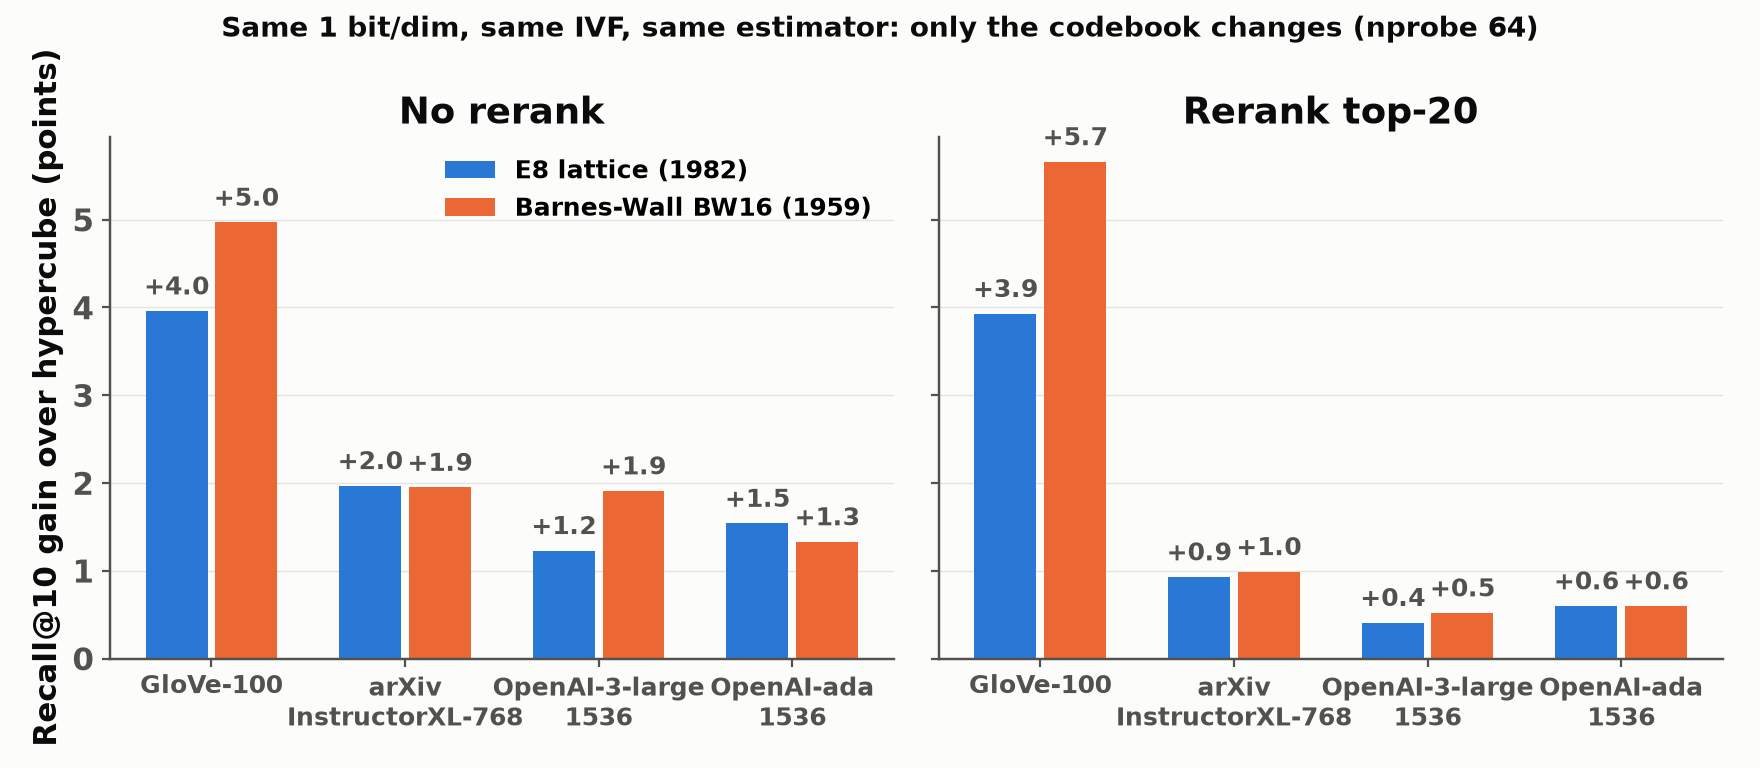
\includegraphics[width=0.9\textwidth]{figs/fig_lattice_gain.png}
\caption{Recall@10 gain of lattice codebooks over the hypercube inside IVF at 1 bit per dimension (50k vectors, nprobe 64), with everything except the codebook held fixed.}
\label{fig:lattice}
\end{figure}

\subsection{The error-isotropy principle}\label{sec:isotropy}
Theorem~\ref{thm:main} depends on $e$ being isotropic in $o^\perp$. This is not a technicality. For a query distribution with covariance $\Sigma_q$, the ranking error is governed by $\mathbb{E}\langle q,e\rangle^2=\mathrm{tr}(\Sigma_q\,\mathbb{E}[ee^\top])$, not by $\mathbb{E}\|e\|^2$. A decoder that minimises $\mathbb{E}\|e\|^2$ on anisotropic data shrinks the error in low-variance directions and leaves it in the high-variance directions that queries share.

We observed this in three settings, which are consistent with the principle though they do not prove it. (a) The Bussgang linear MMSE decoder~\cite{bussgang1952} for sign codes, which costs no storage, halves the reconstruction MSE (0.363 to 0.188) but lowers estimator recall@10 from 0.828 to 0.793 on 229k OpenAI vectors (0.603 to 0.541 on 256 PCA dimensions); rescaling it to be unbiased does not help (0.793).

Measuring the error covariance directly (Supplementary Table~\ref{tab:iso}) supports the mechanism: for every unbiased decoder of Theorem~\ref{thm:main} the ranking error $\mathrm{tr}(\Sigma_qE)$ equals its isotropic prediction to within 1\%, while the Bussgang decoders put 9--16\% of their error in the 50 leading principal directions (3.3\% expected) and are 2.4--4.0$\times$ worse than isotropic along the query distribution. A controlled experiment with synthetic errors (Section~\ref{sec:tests}) isolates the mechanism: at equal MSE, recall varies from 0.49 to 0.97 with the alignment of the error.

(b) At a similar size, cuVS IVF-PQ (trained to minimise MSE, 104\,B/vector) with a 100-candidate refine reaches recall 0.921 on the same data, while a rotated E8 code (98\,B/vector) with a 40-candidate rerank reaches 0.994. (c) At 1 bit per dimension in IVF, a frozen E8 codebook beats a PQ codebook trained on the data (recall 0.773 vs.\ 0.741), and a universal codebook trained only on Gaussian noise matches E8 within 0.3 points. The safe way to exploit anisotropy is therefore bit allocation or truncation, which changes \emph{where} bits go, not how codes are decoded.

\subsection{How many bits does a filter need?}\label{sec:ident}
A first-stage filter does not need to reproduce $x$; it needs to decide whether $\langle q,x\rangle$ exceeds the score of the $k$-th neighbour.

\paragraph{Derivation.} Ingber, Courtade and Weissman~\cite{ingber2015identification} (Theorem~1) consider a source $X\in\mathbb{R}^n$ with i.i.d.\ $\mathcal{N}(0,\sigma^2)$ coordinates, compressed at $R$ bits per coordinate, and queries ``is $\|X-y\|^2\le nD$?'' that must never miss a true match. The smallest achievable rate is
\[
R_{\mathrm{ID}}(D)=\log_2\frac{2\sigma^2}{2\sigma^2-D}\quad\text{bits per coordinate},\qquad 0\le D<2\sigma^2 .
\]
We apply it to unit vectors ($\sigma^2=1/n$, so $\mathbb{E}\|X\|^2=1$) and a cosine threshold $\tau$: $\|x-y\|^2=2-2\langle x,y\rangle\le 2-2\tau$ means $nD=2-2\tau$, i.e.\ $D=(2-2\tau)/n$. Then $2\sigma^2/(2\sigma^2-D)=(2/n)/(2\tau/n)=1/\tau$, so
\[
R_{\mathrm{ID}}=\log_2(1/\tau)\ \text{bits per coordinate},\qquad B_{\mathrm{ID}}=n_{\mathrm{eff}}\log_2(1/\tau)\ \text{bits per vector}.
\]
Real embeddings are neither Gaussian nor isotropic. Our heuristic replaces $n$ by an effective number of independent, equal-variance coordinates $n_{\mathrm{eff}}$; this substitution is not justified by the theorem, which is why we use the result only as a guide.

\paragraph{Numbers and sensitivity.} On 228k OpenAI-1536 vectors (centred and normalised) and 2{,}000 queries, the cosine of the 10th neighbour has median $\tau=0.459$ (10th--90th percentile 0.391--0.560), so $\log_2(1/\tau)=1.12$ bits per effective coordinate. Supplementary Table~\ref{tab:ident} shows that the bound depends strongly on how $n_{\mathrm{eff}}$ is defined. With the participation ratio of the covariance spectrum, $(\sum\lambda_i)^2/\sum\lambda_i^2=124$, it is about 140 bits per vector (101 bits for $k=1$, 180 for $k=100$); with the number of components holding 90\% of the variance it is 486 bits. The participation-ratio value agrees with what we observe: a 138-bit trellis code keeps 96.6\% of the true top-10 in the top 200 candidates, a 202-bit code 98.9\%, while codes well below 140 bits lose candidates quickly (Figure~\ref{fig:ident}). We therefore read the participation-ratio bound as an order-of-magnitude guide for the filter size, not as a limit. Section~\ref{sec:tests} tests it out of sample, on GloVe-100 and for $k=1$ to 100: it lies between the bits needed with 200 and with 2{,}000 candidates in all six cases, but it ignores the candidate budget and does not rank the two datasets reliably.

\section{Trellis Codes for Vector Search}\label{sec:trellis}
\paragraph{Construction.} A bitshift trellis with memory $L$ and $k$ bits per coordinate stores a bit stream $b_0b_1\dots$; the state for coordinate $j$ is the window $s_j=b_{jk}\dots b_{jk+L-1}$ and the reconstruction is $\alpha\,T[s_j]$, where $T$ is a fixed table of $2^L$ values (Gaussian quantiles in a pseudo-random order) and $\alpha$ a global scale. Encoding is a Viterbi search over $2^L$ states that minimises squared error; it is data-oblivious and needs no training. The stream costs $kr+L-k$ bits for $r$ coordinates, so the state overhead is a few percent. We use $k=1$ and $L=10$ for stage-1 codes.

\paragraph{Distortion.} Figure~\ref{fig:dist} compares trellis codes with the per-coordinate Lloyd--Max quantizer used by TurboQuant on a unit Gaussian source. At 1 bit per coordinate the gap to the Shannon bound falls from 1.64\,dB to 0.24\,dB ($L=12$); at 2 bits, from 2.83\,dB to 0.55\,dB.

\begin{figure}[!htbp]
\centering
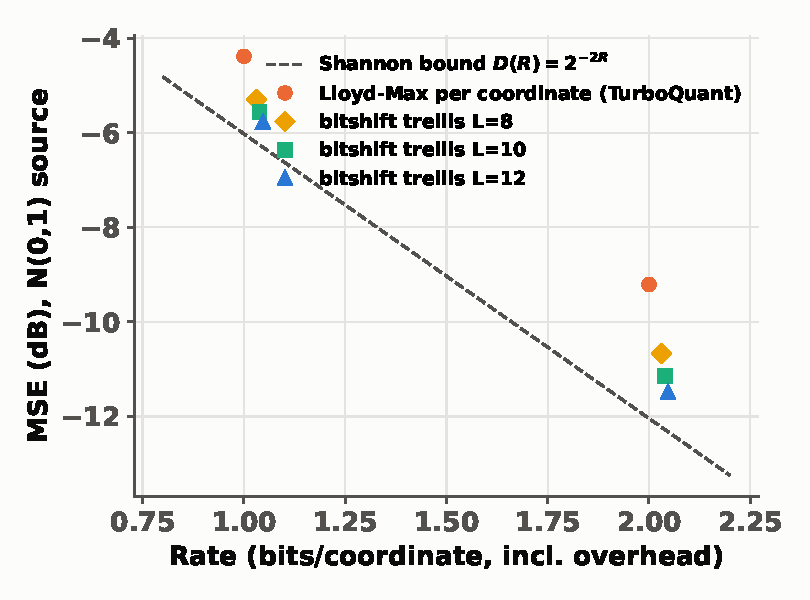
\includegraphics[width=0.68\textwidth]{figs/fig_distortion.pdf}
\caption{Distortion of an N(0,1) source versus rate, including the trellis state overhead. Bitshift trellis codes approach the Shannon bound; the per-coordinate Lloyd--Max quantizer used by TurboQuant stays 1.6 to 2.8\,dB above it.}
\label{fig:dist}
\end{figure}

\paragraph{Real data.} On 229k OpenAI-1536 vectors with the estimator of Theorem~\ref{thm:main} and a full scan, the trellis code raises $c$ from 0.798 to 0.850 (1 bit) and from 0.938 to 0.961 (2 bits), and estimator-only recall@10 from 0.828 to 0.855 and from 0.911 to 0.927, at a 3.6\% (1 bit) and 1.8\% (2 bits) size overhead. With a 40-candidate exact rerank, 1-bit recall rises from 0.9979 to 0.9996.

\paragraph{Identification sizing.} Figure~\ref{fig:ident} shows the fraction of the true top-10 that survives in the top-200 by estimate, as a function of code size. Trellis codes need 25 to 30\% fewer bits than sign codes for the same candidate recall. A 0.5-bit-per-coordinate trellis code on 256 PCA dimensions (138 bits, near the identification estimate) keeps 96.6\% of the true top-10 in the top 200 and 98.7\% in the top 400; a 202-bit code keeps 98.9\% in the top 200.

\begin{figure}[!htbp]
\centering
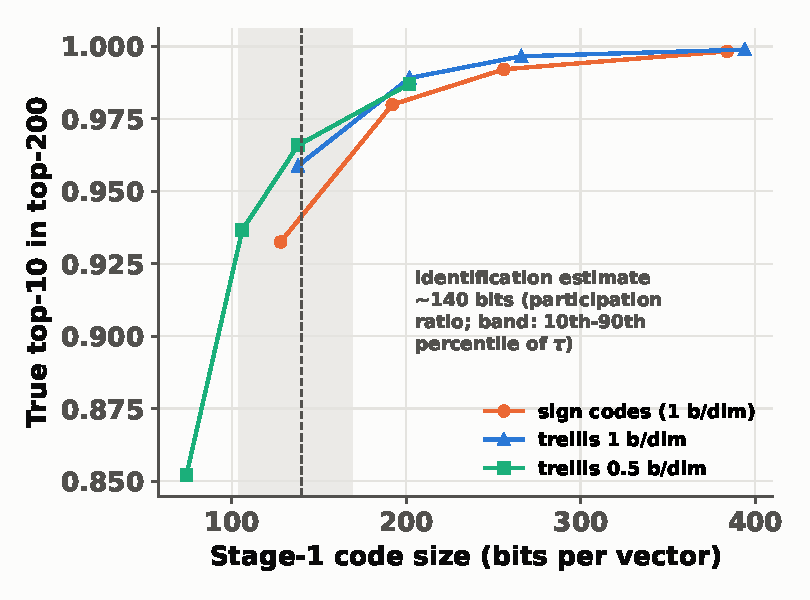
\includegraphics[width=0.68\textwidth]{figs/fig_identification.pdf}
\caption{Candidate recall (true top-10 within the top-200 estimates) versus stage-1 code size on 229k OpenAI-1536 vectors. The dashed line marks the identification-rate estimate with the participation-ratio effective dimension; the band covers the 10th--90th percentile of the neighbour cosine $\tau$.}
\label{fig:ident}
\end{figure}

\paragraph{GPU decoding.} The window property makes decoding embarrassingly parallel: for coordinate $j$ a thread loads two consecutive 32-bit words, shifts out the $L$-bit window and gathers $T[s_j]$ from a 1{,}024-entry table. A Triton~\cite{tillet2019triton} kernel decodes a tile of codes into fp16 registers and multiplies it by a tile of queries with tensor cores, without writing decoded vectors to memory. Encoding is a full Viterbi search over the $2^L=1{,}024$ states. Written as a PyTorch loop over coordinates with the states vectorised, it codes 8{,}500 vectors per second at $R=256$. A fused Triton kernel runs one program per vector, keeps the path costs in a double-buffered scratch row, stores one backpointer bit per state and coordinate (32\,KB per vector) and backtracks in the same kernel; it returns exactly the same paths and codes 477{,}000 vectors per second, 55$\times$ faster, so 10M vectors take about 21\,s of encoding. (A beam search that keeps only the $B$ cheapest paths, which we tried before, trades code quality for speed: $B=16$ codes 48{,}000 vectors per second with $c=0.820$, against $c=0.850$ for the full search.)

\section{FanarVSE}\label{sec:system}
FanarVSE answers a batch of queries in three stages:
\begin{enumerate}
\item \textbf{Stage 1, filter (GPU).} A coarse spherical k-means quantizer with 4{,}096 cells routes each query to $n_p$ cells. Each data vector minus the mean of its cell is projected on the top $R$ principal components, randomly rotated, and coded with a 1-bit trellis code plus a per-vector fp16 scale. A fused kernel returns the exact top $K$ estimates over the probed cells (threshold-and-emit selection, below).
\item \textbf{Stage 2, refine (GPU or host).} Each candidate has a tiered refinement code of its full residual: bits are allocated across groups of principal directions, and each tier is a rotation plus a Lloyd--Max code (TurboQuant-style), stored as bit planes. A second kernel estimates the candidates' scores and their standard deviations from Theorem~\ref{thm:main}, applied per tier.
\item \textbf{Stage 3, error-bar check (RAM or NVMe).} Each candidate gets an interval $\hat s\pm z\sigma$, with $\sigma$ from Theorem~\ref{thm:main} and $\|q\|$ in place of $\|q_\perp\|$, which can only widen it ($z=2$ by default). A candidate is surely in if its lower bound exceeds the $(k{+}1)$-th largest upper bound, and surely out if its upper bound is below the $k$-th largest lower bound. Only the remaining ambiguous candidates are read in full precision; the GPU reads them directly from pinned host memory over PCIe (zero-copy) and scores them.
\end{enumerate}
The first version of FanarVSE (FanarVSE-v1 below) used 64 cells, a 4-bit refinement code on all 1{,}536 coordinates (820\,B/vector) and a different selection kernel, and coded stage 1 relative to one global centre, as did the intermediate engine of Table~\ref{tab:chain}; Section~\ref{sec:eval} reports both, and the measurements of the error bars in Tables~\ref{tab:rot}, \ref{tab:ablation} and~\ref{tab:z} were made with FanarVSE-v1.

\paragraph{Exact block-max selection.} Writing all estimates back to memory would make stage 1 bandwidth-bound. The kernel instead writes only the maximum estimate of each block of 32 vectors, and a second pass rescores the vectors of the top $K$ blocks.
\begin{lemma}
Let $t$ be the $K$-th largest estimate. The $K$ blocks with the largest maxima contain a set of $K$ items whose estimates are the $K$ largest.
\end{lemma}
\begin{proof}
Every block whose maximum exceeds $t$ contains an item with estimate above $t$; there are at most $K-1$ such items, hence at most $K-1$ such blocks. The top $K$ blocks by maximum therefore include all of them, and the remaining selected blocks have maximum equal to $t$. Every item with estimate above $t$ lies in a block of the first kind, and the selected blocks with maximum $t$ supply items with estimate $t$ to complete the set.
\end{proof}
The selection is exact with respect to the estimates; it trades $N$ writes per query for $N/32$ writes plus $32K$ rescored items. FanarVSE-v1 used it directly. Its second pass, which decodes $32K$ items at scattered positions, took more than a third of stage 1 (21 of 57\,ms per 500 queries), and the current engine replaces it with a threshold.

\paragraph{Threshold-and-emit selection.} A first pass computes block maxima only over the $n_1$ nearest of the $n_p$ probed cells; rows of a block that belong to a neighbouring cell are masked. Let $t_0$ be the $r$-th largest of these maxima. A second pass scans all probed cells and appends every item with estimate at least $t_0$ to a per-query buffer through an atomic counter; the top $K$ of the buffer are the candidates.
\begin{lemma}[Threshold selection]\label{lem:thr}
If at least $K$ items of a query's probed cells have estimate at least $t_0$, the top $K$ of its buffer equal the top $K$ of the probed cells. This holds whenever $r\ge K$.
\end{lemma}
\begin{proof}
If at least $K$ probed items have estimates at least $t_0$, the $K$-th largest estimate over the probed cells is at least $t_0$, so every item of the top $K$ is emitted. If $r\ge K$, the $r$ blocks whose maxima are at least $t_0$ are disjoint and each contains a probed item with estimate at least $t_0$ (masked rows do not count), so there are at least $K$ such items.
\end{proof}
The emit pass counts the items it appends, so the condition of the lemma is checked for free, and $t_0$ may be guessed. A smaller first pass makes the guess cheaper, and a higher $t_0$ fills the buffer less. We use $r=0.75K$ with $n_1$ cells holding about $1.1K$ blocks for $K\le400$, and $r=K/2$ with about $0.7K$ blocks for larger $K$ (26--82 cells at $K=200$--$1{,}000$). A query whose buffer received fewer than $K$ items, or more than its 32k entries, is recomputed with $r=K$ and $n_1$ holding $1.5K$ blocks, which the lemma guarantees, or with the block-max selection if the buffer overflows again. The result is exact for every query; the recomputation is needed for fewer than 1\% of queries in our tests, and the guess shortens stage 1 by about a fifth.

\paragraph{Routing, one launch and one decode.} Codes are sorted by cell. Many small cells keep the scanned fraction of the data close to what a query needs, but launching one kernel per cell, as FanarVSE-v1 did, costs more than the scan once there are thousands of cells. All (cell, block) pairs that a batch probes therefore form one flat work list, processed by a single launch; each program decodes its block of 32 trellis codes once into registers and multiplies it with every tile of queries that probes the cell. With 4{,}096 cells, $n_p=768$ and a batch of 500 queries, stage 1 takes 25\,ms, against 37\,ms when each block is decoded once per tile of 32 queries (20\,ms with the guessed threshold and fp16 queries described above). In the lean variant, stage 2 runs on the CPU from host memory and overlaps with stage 1 of the next batch; only candidate ids cross PCIe.

\paragraph{Cell-residual stage 1.} Stage 1 codes $x-m_c$, where $m_c$ is the mean of the cell $c$ that holds $x$, and estimates $\langle q,x\rangle$ by $\langle q,m_c\rangle$ plus the trellis estimate of $\langle q,x-m_c\rangle$. Coding the residual from the coarse centroid is standard in inverted-file indexes (IVFADC~\cite{jegou2011pq}, IVF-RaBitQ~\cite{shi2026ivfrabitq}); our earlier engines coded the residual from one global centre and used the cells only for routing. The cell residual has less energy (the mean squared norm falls from 1.00 to 0.68 on the OpenAI vectors, from 0.52 to 0.25 on SigLIP image embeddings and from 0.93 to 0.39 on DINOv2 image embeddings), so the same 1-bit code ranks better: with the trellis encoder and $R=256$, the share of the true top-10 among the top 200 estimates of 128 probed SigLIP cells rises from 0.977 to 0.994, and on DINOv2 ($R=512$, 64 probed cells) 100 candidates of the cell-residual code keep more of them than 200 of the global one (0.991 against 0.988). We keep the global principal basis; a basis computed from the cell residuals changed these numbers by at most 0.002. The constant $\langle q,m_c\rangle$ depends on the query and the cell, so it cannot be folded into the per-query offset of the kernels. Each (cell, query) pair of the sorted work list has a unique index, and the kernels read the constant from an array in that order, gathered from one matrix product $QM^\top$ of the queries with the fp16 table of cell means. The same table routes the queries: the centroid of a spherical k-means cell is the normalised mean of its members, so we rank cells by $\langle q,m_c\rangle/\|m_c\|$ and keep no separate centroid table. Stage 2 still codes the residual from the global centre: Theorem~\ref{thm:main} holds for any centre, and coding stage 2 from the cell mean too cut the exact reads from 6.6 to 5.3 per query on OpenAI and from 29 to 16.5 on SigLIP, but at equal or 5\% lower throughput on the GPU, because the constant must then be computed in fp32 for every candidate; it is an option for the NVMe tier, where reads cost more.

\paragraph{Tiered refinement.} The refinement code spends bits where the residuals have variance. In the principal basis of the residuals, with eigenvalues $\lambda_i$, the coordinates are split into groups of 32, and $b_g\ge1$ bits per coordinate are assigned to group $g$ greedily to minimise $\sum_g\big(\sum_{i\in g}\lambda_i\big)D(b_g)$, where $D(b)$ is the Lloyd--Max distortion of a unit Gaussian at $b$ bits (reverse water-filling with the quantizer's real distortions; bit allocation is prior art~\cite{saq2025}). Consecutive groups with the same width form a tier; at 3{,}840 bits per vector this gives six tiers: 7 bits on the 32 leading directions, then 5, 4, 3 and 2 bits on 96, 256, 320 and 320 directions, and 1 bit on the last 512. Each tier $t$, with coordinates $o_t$, is coded as in Theorem~\ref{thm:main}: its own Haar rotation, a Lloyd--Max code, the per-vector factor $\|o_t\|/c_t$ and its $\sigma_t$, in fp16. The score estimate is $\langle q,\mu\rangle+\sum_t\widehat{\langle q_t,o_t\rangle}$, where $\mu$ is the global centre. One kernel computes all tiers' contributions and $\sigma$ for a tile of candidates, with each tier's width and bit count fixed at compile time; the tier rotations are applied to the queries by a single block-diagonal matrix product. Since the PCA basis and the tier rotations fold into one $d\times d$ matrix, the query-side cost is that of a single rotation; sharing one rotation among tiers would save nothing and would correlate the tier errors, which Corollary~\ref{cor:tier} needs to be independent.
\begin{corollary}[Tiered codes]\label{cor:tier}
The tiered estimate is unbiased, its error variance is $\sum_t\|q_{t\perp}\|^2(1-c_t^2)/(c_t^2(d_t-1))$, and with $\sigma^2$ equal to this sum or to any upper bound of it (such as the engine's $\sum_t\|q_t\|^2\sigma_t^2$), $P(|\hat s-s|>z\sigma)\le2e^{-z^2/2}$.
\end{corollary}
\begin{proof}
Each tier satisfies Theorem~\ref{thm:main} with its own independent rotation, so the tier errors are independent and unbiased, and the variances add. By Corollary~\ref{cor:law} each standardised tier error is $\sqrt{m}\,u_1$ for a uniform $u$ on $S^{m-1}$; its odd moments vanish and its even moments are at most those of a standard Gaussian, so its moment-generating function is at most $e^{\lambda^2/2}$. The sum is therefore sub-Gaussian with variance proxy $\sigma^2$, and the Chernoff bound gives the tail.
\end{proof}
The exact law of a tier is no longer the law of the sum, so for the tiered code we use this sub-Gaussian bound for certified settings.

\paragraph{Why error bars.} With any refinement code alone, recall saturated near 0.94 to 0.966 on 998k vectors even when $c=0.995$: the estimator's error (about 0.002) is comparable to the gap between the 10th and 11th scores. More bits do not fix this, but knowing the error does. On 998k vectors the error-bar test reaches the candidate-set ceiling (recall 0.9955 at $n_p=32$, $K=100$) with 57 exact reads per query from 1-bit codes alone, 11.7 with a 3-bit refinement and 5.7--5.9 (p99: 15--16, maximum 22 over 2{,}000 queries) with a 4-bit refinement.

\paragraph{A coverage guarantee.} The test is exact whenever the intervals are right:
\begin{lemma}[Coverage implies exactness]\label{lem:cov}
If every candidate's interval contains its true score, stage 3 returns exactly the top-$k$ of the candidate set.
\end{lemma}
\begin{proof}
Let $s_j\in[\ell_j,h_j]$ for all candidates. (a) At most $k$ candidates are surely in: if $k{+}1$ had $\ell_j$ above the $(k{+}1)$-th largest upper bound, they would have $k{+}1$ upper bounds above it. (b) A surely-in candidate $i$ has $s_i\ge\ell_i>h_{(k+1)}\ge s_{(k+1)}$, so it is in the true top-$k$. (c) A surely-out candidate $i$ has $s_i\le h_i<\ell_{(k)}\le s_{(k)}$, so it is not. Hence the true top-$k$ lies among the surely-in and ambiguous candidates; the latter are scored exactly, and the result is the surely-in set completed by the best ambiguous ones.
\end{proof}
With the union bound and Corollary~\ref{cor:law}, the probability (over the random rotation) that a query's result differs from the exact top-$k$ of its $K$ candidates is at most $K\,P(|Z|>z)$. For $K=400$ this is 0.5\% at $z=4.36$ and 0.1\% at $z=4.69$; for comparison, Chebyshev's and Cantelli's inequalities~\cite{cantelli1928}, which use the variance alone, need $z\approx10$ for a 1\% guarantee per interval. Section~\ref{sec:eval} measures what each choice costs.

\paragraph{Zero-copy exact reads.} The full fp16 vectors stay in host RAM, in page-locked memory that the GPU can address through unified virtual addressing. A kernel with one program per candidate exits unless the candidate is ambiguous, and otherwise reads its 3{,}072\,B row over PCIe and computes the exact score. No candidate ids travel to the CPU and no host gather is needed: for 3{,}200 rows this takes 1.05\,ms against 3.04\,ms for a CPU gather followed by a copy to the GPU. Host RAM, not GPU memory, holds the vectors, so the GPU footprint is unchanged.

\paragraph{Small batches, one CUDA graph and NVMe.} For up to 32 queries FanarVSE uses fixed-grid stage-1 kernels that need no work list, and large batches use a fixed work list with one program for every (cell, block) of the index. Stages 1--3 then contain no host synchronisation, so every search is one CUDA graph replay; a query that fails the count check is recomputed on the general path, so every result stays exact. Full vectors can also live on an NVMe drive, read by a small C library with overlapped I/O and up to 128 requests in flight (127k random 4\,KB reads per second). Supplementary Note~\ref{sn:eng} gives the details.

\paragraph{Memory accounting.} We count every byte the index keeps on the GPU, measured by summing the device tensors of the built index. With $R=256$, stage 1 stores nine 32-bit words per vector (the 266-bit trellis path, word-aligned), an fp16 scale and an int32 id, 42\,B per vector. The shared tables take 23.6\,MB: the fp16 cell means, which also route (12.6\,MB), the query-side rotation of the tiered code (9.4\,MB), the projection matrix (1.6\,MB) and the trellis table; that is 24\,B per vector at 998k, and less as $N$ grows. The lean variant therefore keeps 66\,B per vector on the GPU. The tiered refinement adds 504\,B (3{,}840 bits plus an fp16 factor and $\sigma_t$ for each of the six tiers), for 570\,B per vector in total; with $R=384$ stage 1 stores 58\,B per vector and the total is 586\,B. Earlier versions of this accounting undercounted the shared tables; the intermediate engine of Table~\ref{tab:chain} also held int64 ids, an fp32 centroid table and the build-time PCA basis and tier rotations (48\,MB of tables), which the final engine moves off the GPU. FanarVSE-v1's 4-bit refinement added 772\,B (820\,B in total). Full vectors (3{,}072\,B in fp16) live in host RAM or on NVMe and are read only for ambiguous candidates. In the lean variant the refinement code also stays in pinned host RAM, packed as one contiguous 512-byte record per vector (all tiers' bit planes, then the per-tier factors), and the fused stage-2 kernel reads the records of the candidates over PCIe by zero-copy, as stage 3 reads full vectors; only stage 1 and the shared tables, 66\,B per vector at 998k (82\,B with $R=384$), stay on the GPU. A contiguous record matters: with the bit planes of each tier stored separately, the many small PCIe reads made the lean variant 1.8$\times$ slower.

\subsection{Throughput mode}\label{sec:tmode}
When many queries arrive together, memory per vector matters less than queries per second. At a batch of 4{,}000, stage 1 of the default engine takes 13.2\,\textmu s per query and stage 2 more than 9, against 2.0 for routing and 1.9 for stage 3: decoding trellis codes and gathering refinement codewords dominate, not the exact reads. FanarVSE-T, an optional throughput mode, changes three parts and keeps the rest (routing, threshold-and-emit selection with its count check and recomputation, error bars, zero-copy stage 3).

\paragraph{An int8 first stage.} Each cell residual $x-m_c$ is projected on the same 256 principal directions and stored as int8, scaled per vector so that its largest coordinate is $\pm127$, with an fp32 scale: 260\,B instead of the 42\,B of the trellis code. The query is projected and quantised in the same way, and a Triton kernel scores code blocks against query tiles with int8 tensor cores; there is nothing to decode. The finer code ranks better: among the top 100 estimates over 384 probed cells it keeps 99.0\% of the true top 10 (99.3\% among the top 400, against 99.2\% for the trellis code), so $K=150$--400 candidates suffice where the default needs 400--800. Stage 1 does not need an unbiased estimate, only a ranking, and its selection stays exact (Lemma~\ref{lem:thr}): the first pass sets $r=0.6K$, the buffer holds 3{,}072--8{,}192 entries, and a query that fails the count check is recomputed with $r=K$ and a 65{,}536-entry buffer.

\paragraph{Refinement scored by lookup tables.} The tiered code keeps its tiers and bit widths but replaces each tier's Lloyd--Max codebook by a uniform one, with levels $\Delta_b\,(j-(2^b-1)/2)$ and $\Delta_b$ chosen to minimise the distortion of a unit Gaussian. The codeword is then affine in its bit planes $\beta_p$, so $\langle q_t,\bar o_t\rangle=\Delta_b\big(\sum_p 2^{b-1-p}\langle q_t,\beta_p\rangle-\tfrac{2^b-1}{2}\sum_i q_{t,i}\big)$, and each $\langle q_t,\beta_p\rangle$ is a sum of lookups in 16-entry tables, one per four coordinates, built once per query in fp16 and shared by every plane and candidate. The kernel computes the same estimates as a codeword gather. Theorem~\ref{thm:main} holds for any codebook, so the estimate stays unbiased and Corollary~\ref{cor:tier} applies with the uniform code's $c_t$; the coarser codebook adds 0.24 exact reads per query at $z=2$ (6.64 to 6.88) and leaves recall unchanged. Stage 2 also scores only the candidates whose stage-1 estimate lies within $\delta=0.07$ of the query's 10th-best stage-1 estimate; the others cannot plausibly reach the top 10 and are dropped. This rule is measured, not proved: at $n_p=384$ it lowered recall from 0.9921 to 0.9919.

\paragraph{Cheaper routing and smaller intervals.} The table of cell means is stored normalised, so routing is a top-$n_p$ over one fp16 product, and the stage-1 constants are recovered as $\langle q,m_c/\|m_c\|\rangle\,\|m_c\|$ from a 16\,KB table of norms; (query, cell) pairs are grouped with one stable sort of 32-bit keys. The error bars use $z=1.25$, which cuts the exact reads from 6.9 to 4.2 per query and costs 0.0003 of recall (0.9921 to 0.9918 at $n_p=384$); above recall 0.997 we use $z=1.5$ and score all candidates.

\paragraph{Memory.} FanarVSE-T keeps 768\,B per vector on the GPU (260\,B of stage-1 code and scale, the 504\,B tiered code and a 4-byte id) and 18.9\,MB of shared tables (normalised cell means, fp16 query-side rotation of the tiered code, PCA basis), 787\,B per vector at 998k, measured as for the default engine: 1.4$\times$ the default's 570\,B and 4.1$\times$ less than CAGRA. Supplementary Note~\ref{sn:tput} gives the gain of each change and the variants that did not help.

\subsection{Which guarantee holds where}\label{sec:modes}
Table~\ref{tab:modes} collects, for each stage and mode, what is exact, what is bounded and what is only measured. Two choices apply to every mode. First, the engine's $\sigma$ uses $\|q\|$ (per tier, $\|q_t\|$) in place of $\|q_\perp\|$, which can only widen the interval. Second, every probability statement is over the random rotation and assumes a Haar rotation; FanarVSE uses dense Haar rotations, and for structured rotations we have only the measurements of Table~\ref{tab:rot}.

\begin{table}[!htbp]
\caption{Guarantees by stage and operating mode. ``Exact'': holds deterministically for the estimates; ``bound'': holds in probability over a Haar rotation; ``measured'': no proof, empirical only.}
\label{tab:modes}
\small
\begin{tabular}{p{3.3cm}p{5.2cm}p{6.9cm}}
\toprule
Stage / mode & Statement & Status \\
\midrule
Stage 1, selection & Candidates are the top $K$ estimates of the probed cells & Exact (Lemmas~\ref{lem:thr} and block-max; count check, recomputation on failure) \\
Stage 1, routing and code & True neighbours are among the candidates & Measured (candidate-set ceiling) \\
Stage 1, graph mode & Candidates are the best $K$ entries of the beam & Measured only (no exact selection; Table~\ref{tab:graph}) \\
Stage 2, throughput mode & Uniform tier codebooks: as for the tiered code; candidates dropped by the $\delta$ rule are not in the top $k$ & Bound as for the tiered code; the $\delta$ rule is measured only (Section~\ref{sec:tmode}) \\
Stage 2, single code (FanarVSE-v1) & Estimate unbiased; $Z$ follows Corollary~\ref{cor:law} & Bound; per query $K\,P(|Z|>z)$ (0.5\% at $z=4.36$, $K=400$) \\
Stage 2, tiered code & Estimate unbiased; sub-Gaussian tail & Bound; per query $2K e^{-z^2/2}$ (0.49\% at $z=4.9$, $K=400$) \\
Stage 2, tiered, certified plug-in & Same, with $\sigma'\le$ engine $\sigma$ & Bound (Corollary~\ref{cor:lcb}); per query $2K(Te^{-z_1^2/2}+e^{-z_2^2/2})$ (0.46\% at $z_1=5.6$, $z_2=4.95$) \\
Stage 3, $z=2$ (default) & Result equals the top $k$ of the candidates & Measured (equal to the ceiling to within 0.0002 in every run at 998k, 0.0005 on the other sets); not certified \\
Stage 3, certified $z$ & Same & Bound, via Lemma~\ref{lem:cov} and the line above \\
Stage 3, structured rotations & Same & Measured only (Table~\ref{tab:rot}) \\
\bottomrule
\end{tabular}
\end{table}

\paragraph{Tightening $\sigma$.} Plugging the stage-2 estimate and a stored residual norm into $\|q_\perp\|$ cuts the reads from 6.6 to 5.6 per query at $z=2$ at unchanged recall. A certified variant that plugs in a lower confidence bound per tier (Supplementary Corollary~\ref{cor:lcb}) cuts them from 17.9 to 15.5 at a per-query bound of 0.46\%. We keep $\|q\|$ as the default (Supplementary Note~\ref{sn:sigma}).

\paragraph{Euclidean distance.} For L2 search, $\|q-x\|^2=\|q\|^2+\|x\|^2-2\langle q,x\rangle$, and with $\|x\|$ stored per vector (2\,B in fp16) the ranking is by $\langle q,x\rangle-\|x\|^2/2$. The inner-product estimate and its interval carry over unchanged, shifted by a known constant per candidate, so stages 1--3, the lemmas and the bounds apply as stated. We did not evaluate L2 datasets.

\paragraph{Choosing the parameters.} Supplementary Note~\ref{sn:params} gives an order in which to set $R$, the refinement size, the number of cells, $K$, $n_p$ and $z$.

\section{Evaluation}\label{sec:eval}
\subsection{Setup}
\paragraph{Hardware and software.} One laptop with an NVIDIA RTX 3050 (6\,GB, Ampere), a 16-thread CPU, 16\,GB of RAM and a Micron NVMe drive. FanarVSE runs on native Windows (PyTorch 2.6, Triton 3.2); the GPU baselines run in WSL2 Ubuntu on the same GPU and driver: FAISS-GPU 1.14 and cuVS 26.10 (CAGRA, IVF-PQ and IVF-RaBitQ). cuVS 26.10 ships IVF-RaBitQ only through its C++ API, so we call the library's \texttt{build} and \texttt{search} functions directly from Python (through \texttt{ctypes}) and verified the binding against brute force. All cuVS baselines use an RMM memory pool, which removes per-call allocation costs that otherwise dominate small batches.

\paragraph{Tuning the baselines.} For CAGRA we swept the internal top-$k$ (itopk) from 64 to 1024, graph degrees 32 and 64, and all four search algorithms (auto, single-CTA, multi-CTA, multi-kernel), and we report the best configuration at each recall. At itopk 384--512 the automatic choice was up to 2.3$\times$ slower than multi-CTA, so earlier CAGRA numbers in this regime were pessimistic. For IVF-RaBitQ we swept 2--9 bits per dimension, 1{,}024 and 4{,}096 lists, 16 to 2{,}048 probes and its four scan modes; 9 bits with 4{,}096 lists is best above recall 0.98. GPU memory for IVF-RaBitQ is measured as the drop in free device memory during the build.

\paragraph{Same operating system for both?} FanarVSE itself runs within 2\% of its native-Windows throughput in WSL2, with the same PyTorch and Triton versions, so the operating-system split does not favour it (Supplementary Table~\ref{tab:os}).

\paragraph{Data.} (a) 998k OpenAI text-embedding-ada-002 vectors (1536 dims) from DBpedia, 2{,}000 held-out queries; (b) a 228{,}772-vector subset of the same data; (c) GloVe-100 (1{,}183{,}514 vectors, angular); (d) five more sets, two of them image embeddings and one with 2.25M vectors, described in Section~\ref{sec:more}. Ground truth is exact inner-product top-10 and top-100, computed on the GPU in fp32. All engines use the same queries and ground truth.

\paragraph{Metrics.} Recall@$k$ and queries per second (QPS) at a batch of 500 queries unless stated, end to end including reranking and the CPU/SSD stages. Each configuration is warmed up once and then timed three times; we report the mean and standard deviation. GPU memory is reported per vector, including all codes and per-vector factors. CAGRA and FAISS-GPU use fp16 datasets at 998k because fp32 does not fit in 6\,GB alongside the CAGRA graph.

\subsection{One million OpenAI vectors}
Table~\ref{tab:1m} and Figure~\ref{fig:1m} give the main result.

\textbf{Around recall 0.95,} CAGRA's fastest point is 26.7k QPS at 0.948 and IVF-RaBitQ reaches 15.0k QPS at 0.971; FanarVSE runs at 39.6k QPS at 0.957 and 29.7k at 0.978. We did not measure the engines below 0.945.

\textbf{From 0.95 to 0.998 FanarVSE is the fastest index and uses the least memory.} At 0.992 it runs at 22{,}649 QPS against 4{,}421 for CAGRA at 0.991 (5.1$\times$) and 7{,}466--8{,}079 for IVF-RaBitQ at 0.992 (2.8--3.0$\times$; 8{,}079 with an RMM pool). At 0.994 it is 6.4$\times$ faster than CAGRA; at 0.997 (17{,}911 QPS) it is 3.9$\times$ faster than IVF-RaBitQ at 0.9965 and 10$\times$ faster than CAGRA, and at 0.998 (13{,}674 QPS) 6.4$\times$ and 15$\times$. It uses 570\,B/vector, 3.2$\times$ less GPU memory than IVF-RaBitQ (1{,}851\,B) and 5.6$\times$ less than CAGRA. With at most 1{,}101\,B/vector (5 bits) IVF-RaBitQ does not exceed 0.983.

\textbf{Above 0.998 only FanarVSE and brute force remain:} CAGRA's best is 0.998 (891 QPS, degree 64) and IVF-RaBitQ's 0.998 (2{,}151 QPS, 2{,}048 probes), where its 9-bit estimator saturates. With $R=256$ FanarVSE reaches 0.999 at 12{,}057 QPS, 7.5$\times$ the throughput of fp16 brute force (1{,}598 QPS). With $R=384$ (586\,B/vector) it reaches 0.9995 at 6{,}067 QPS and 0.9998, the recall of fp16 brute force, at 3{,}746 QPS: 2.3$\times$ the throughput of brute force with 5.2$\times$ less GPU memory. At this point stage 1 keeps every true neighbour (candidate-set ceiling 1.000); the remaining 0.0002 is lost because the exact scores are computed from fp16 vectors, as in fp16 brute force.

\textbf{With 66\,B/vector on the GPU} (FanarVSE-lean: refinement records and full vectors in pinned host RAM, read by zero-copy), FanarVSE reaches 0.992 at 11{,}366 QPS, 1.4--1.5$\times$ IVF-RaBitQ at 0.992 (7{,}466--8{,}079) with 28$\times$ less GPU memory, and 0.998 at 6{,}206 QPS; with 82\,B/vector ($R=384$) it reaches 0.999 at 5{,}283 QPS and 0.9998 at 2{,}521 QPS. With the full vectors on the NVMe drive instead of host RAM, read by the asynchronous reader, the 66\,B variant reaches 0.992 at 9{,}057 QPS, still faster than IVF-RaBitQ, and 0.998 at 5{,}475 QPS, and the 82\,B variant 0.9998 at 2{,}348 QPS, 1.5$\times$ fp16 brute force with 37$\times$ less GPU memory. The only other index in that memory range, cuVS IVF-PQ with a 100--200-candidate refine (104\,B/vector), stays below 0.92.

Our grid over $n_p\in\{64,\dots,3{,}072\}$ and $K\in\{100,200,400,800,1{,}200\}$ gives the FanarVSE frontier in Figure~\ref{fig:1m}; in every configuration recall equals the candidate-set ceiling to within 0.0002, so the error-bar stage never lost a neighbour that stage 1 had found.

\begin{table}[!htbp]
\caption{998k OpenAI-1536 vectors, one RTX 3050, $k=10$, batch 500. GPU memory per vector includes all codes and per-vector factors and, for FanarVSE, the shared tables (24\,B/vector). QPS is the mean $\pm$ standard deviation of three timed runs. FanarVSE and FanarVSE-lean use 4{,}096 cells, the cell-residual stage 1 and the tiered refinement (on the GPU, or in host RAM for FanarVSE-lean); $n_p$ cells probed, $K$ candidates, $R=256$ unless stated. MC: multi-CTA search.}
\label{tab:1m}
\small
\setlength{\tabcolsep}{4pt}
\begin{tabular}{lrrr}
\toprule
Engine & GPU B/vec & Recall@10 & QPS \\
\midrule
FAISS-GPU flat fp16 & 3{,}072 & 0.9998 & 1{,}598 $\pm$ 8 \\
CAGRA deg32, itopk 64 & 3{,}200 & 0.948 & 26{,}697 $\pm$ 128 \\
CAGRA deg32, itopk 128 & 3{,}200 & 0.971 & 14{,}827 $\pm$ 35 \\
CAGRA deg32, itopk 256 & 3{,}200 & 0.984 & 7{,}898 $\pm$ 6 \\
CAGRA deg32, itopk 384, MC & 3{,}200 & 0.991 & 4{,}421 $\pm$ 4 \\
CAGRA deg32, itopk 512, MC & 3{,}200 & 0.994 & 3{,}368 $\pm$ 2 \\
CAGRA deg32, itopk 1024 & 3{,}200 & 0.997 & 1{,}734 $\pm$ 0 \\
CAGRA deg64, itopk 1024 & 3{,}328 & 0.998 & 891 $\pm$ 0 \\
IVF-RaBitQ 5 bit, 1{,}024 lists, $n_p$=256 & 1{,}101 & 0.983 & 5{,}721 $\pm$ 16 \\
IVF-RaBitQ 9 bit, 4{,}096 lists, $n_p$=128 & 1{,}851 & 0.971 & 14{,}970 $\pm$ 119 \\
IVF-RaBitQ 9 bit, 4{,}096 lists, $n_p$=256 & 1{,}851 & 0.986 & 9{,}928 $\pm$ 49 \\
IVF-RaBitQ 9 bit, 4{,}096 lists, $n_p$=384 & 1{,}851 & 0.992 & 7{,}466 $\pm$ 35 \\
IVF-RaBitQ 9 bit, 4{,}096 lists, $n_p$=768 & 1{,}851 & 0.9965 & 4{,}578 $\pm$ 20 \\
IVF-RaBitQ 9 bit, 4{,}096 lists, $n_p$=2048 & 1{,}851 & 0.998 & 2{,}151 $\pm$ 1 \\
cuVS IVF-PQ pq96, $n_p$=128, refine 100 & 104 & 0.886 & 1{,}458 $\pm$ 5 \\
cuVS IVF-PQ pq96, $n_p$=256, refine 200 & 104 & 0.918 & 651 $\pm$ 2 \\
\midrule
FanarVSE $n_p$=128, $K$=100 & 570 & 0.957 & 39{,}555 $\pm$ 52 \\
FanarVSE $n_p$=192, $K$=200 & 570 & 0.978 & 29{,}679 $\pm$ 29 \\
FanarVSE $n_p$=256, $K$=200 & 570 & 0.982 & 28{,}684 $\pm$ 108 \\
FanarVSE $n_p$=384, $K$=200 & 570 & 0.988 & 26{,}484 $\pm$ 243 \\
FanarVSE $n_p$=384, $K$=400 & 570 & 0.992 & 22{,}649 $\pm$ 69 \\
FanarVSE $n_p$=512, $K$=400 & 570 & 0.994 & 21{,}513 $\pm$ 91 \\
FanarVSE $n_p$=768, $K$=400 & 570 & 0.996 & 19{,}624 $\pm$ 29 \\
FanarVSE $n_p$=1024, $K$=400 & 570 & 0.997 & 17{,}911 $\pm$ 35 \\
FanarVSE $n_p$=1024, $K$=800 & 570 & 0.998 & 13{,}674 $\pm$ 37 \\
FanarVSE $n_p$=1536, $K$=800 & 570 & 0.999 & 12{,}057 $\pm$ 32 \\
FanarVSE $R$=384, $n_p$=1536, $K$=800 & 586 & 0.9995 & 6{,}067 $\pm$ 4 \\
FanarVSE $R$=384, $n_p$=2048, $K$=1{,}200 & 586 & 0.9997 & 4{,}684 $\pm$ 3 \\
FanarVSE $R$=384, $n_p$=3072, $K$=1{,}200 & 586 & 0.9998 & 3{,}746 $\pm$ 2 \\
\midrule
FanarVSE-lean $n_p$=192, $K$=100 & \textbf{66} & 0.965 & 27{,}156 $\pm$ 90 \\
FanarVSE-lean $n_p$=256, $K$=200 & \textbf{66} & 0.982 & 17{,}582 $\pm$ 216 \\
FanarVSE-lean $n_p$=384, $K$=400 & \textbf{66} & 0.992 & 11{,}366 $\pm$ 19 \\
FanarVSE-lean $n_p$=512, $K$=400 & \textbf{66} & 0.994 & 11{,}077 $\pm$ 41 \\
FanarVSE-lean $n_p$=768, $K$=800 & \textbf{66} & 0.9975 & 6{,}382 $\pm$ 11 \\
FanarVSE-lean $n_p$=1024, $K$=800 & \textbf{66} & 0.998 & 6{,}206 $\pm$ 6 \\
FanarVSE-lean $R$=384, $n_p$=1536, $K$=400 & \textbf{82} & 0.999 & 5{,}283 $\pm$ 10 \\
FanarVSE-lean $R$=384, $n_p$=3072, $K$=1{,}200 & \textbf{82} & 0.9998 & 2{,}521 $\pm$ 1 \\
FanarVSE-lean, NVMe, $n_p$=256, $K$=200 & \textbf{66} & 0.982 & 12{,}969 $\pm$ 99 \\
FanarVSE-lean, NVMe, $n_p$=384, $K$=400 & \textbf{66} & 0.992 & 9{,}057 $\pm$ 10 \\
FanarVSE-lean, NVMe, $n_p$=512, $K$=400 & \textbf{66} & 0.994 & 8{,}854 $\pm$ 19 \\
FanarVSE-lean, NVMe, $n_p$=1024, $K$=800 & \textbf{66} & 0.998 & 5{,}475 $\pm$ 23 \\
FanarVSE-lean, NVMe, $R$=384, $n_p$=1536, $K$=400 & \textbf{82} & 0.999 & 4{,}601 $\pm$ 5 \\
FanarVSE-lean, NVMe, $R$=384, $n_p$=3072, $K$=1{,}200 & \textbf{82} & 0.9998 & 2{,}348 $\pm$ 3 \\
\bottomrule
\end{tabular}
\end{table}

\begin{figure}[!htbp]
\centering
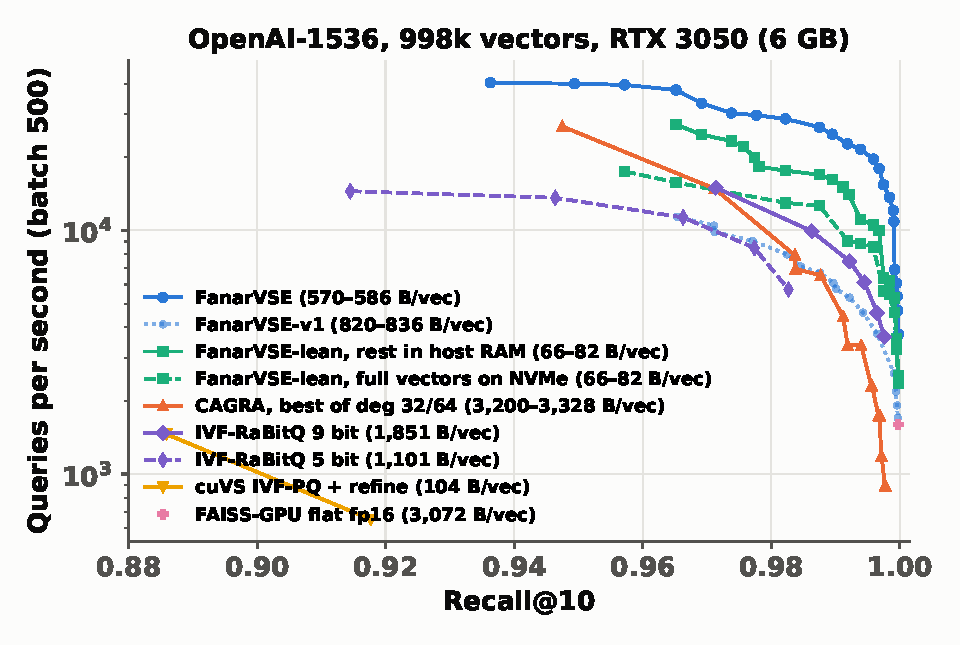
\includegraphics[width=0.85\textwidth]{figs/fig_recall_qps_1m.pdf}
\caption{Recall@10 versus throughput on 998k OpenAI-1536 vectors, same GPU, queries and ground truth. Each curve is the best configuration at each recall (FanarVSE: grid over $n_p$, $K$ and $R\in\{256,384\}$ with 4{,}096 cells; FanarVSE-v1: grid over $n_p$ and $K$ with 64 cells plus the $R=384$ full scan; CAGRA: best of degree, itopk and search algorithm). Legends give GPU memory per vector.}
\label{fig:1m}
\end{figure}

\paragraph{Lychee.} Lychee~\cite{zhao2026lychee} targets the same regime (recall 0.999--0.9999 with few full-precision reads) but no implementation was available to us, so we cannot compare it on our hardware. The two designs are complementary rather than competing: Lychee keeps full vectors in the inverted lists and certifies exactness with respect to IVF-Flat over the probed lists, using geometric bounds; FanarVSE keeps only 8--586\,B/vector on the GPU and bounds the error of a compressed estimate. Lychee's anchor bounds could screen FanarVSE's stage-1 candidates, and FanarVSE's error law could tighten Lychee's screening when vectors are compressed.

\paragraph{Build time.} CAGRA builds in 27\,s (degree 32) and 33\,s (degree 64); IVF-RaBitQ in 11--25\,s with 1{,}024 lists and 82\,s with 4{,}096 lists; cuVS IVF-PQ took 37 to 165\,s in different runs. With the fused encoder of Section~\ref{sec:trellis}, FanarVSE builds from scratch in 28\,s ($R=256$) and 31\,s ($R=384$): 8.3--8.9\,s for a first stage-1 encoding with its PCA, rotation and scale search, 4\,s for the tiered refinement, 12\,s for the 4{,}096-cell quantizer and 4.3--5.6\,s to re-encode stage 1 against the cell means. The rebuilt index gives the same recall as the measured one (0.9959 at $n_p=768$, $K=400$). With the PyTorch encoder the build took 122 to 135\,s.

\paragraph{Where the speed comes from.} Table~\ref{tab:chain} adds the changes from FanarVSE-v1 to the final engine one at a time, with the same queries and ground truth. The tiered refinement makes stage 2 faster and the index 33\% smaller at the same recall, at the cost of 0.8 more exact reads per query. Moving from 64 to 4{,}096 cells lets a query scan a smaller fraction of the data for the same candidate recall (768 of 4{,}096 cells, 19\% of the data, against 32 of 64), which pays only once all cells are processed by one launch. The threshold removes the rescoring pass of the block-max selection, decoding each block once removes repeated trellis decoding, scoring the ambiguous rows on the GPU removes the CPU stage, the guessed threshold and the fused refinement kernel shorten stages 1 and 2, and zero-copy reads remove the host gather. Coding stage 1 from the cell mean raises recall at the same $n_p$ and $K$ (0.9929 to 0.9957) at 3\% lower throughput, so at equal recall it is faster (Table~\ref{tab:1m}); the synchronisation-free batch path adds 7\%, and the single table of cell means (which also removes a matrix product) with the register-built decoder in the fixed-grid kernels another 13\%. Recall is unchanged by the other steps except the routing (0.9922 to 0.9929); overall, throughput rises 3.7$\times$ and recall from 0.9922 to 0.9959.

\begin{table}[!htbp]
\caption{From FanarVSE-v1 to the final engine, one change at a time (998k vectors, $k=10$, batch 500, $z=2$, $K=400$; mean $\pm$ standard deviation of three timed runs). B/vec: per-vector GPU bytes (codes, factors, ids); the shared tables add 11\,MB for FanarVSE-v1, 48\,MB for the intermediate 4{,}096-cell engines (fp32 centroids, build-time PCA basis and rotations), 60\,MB with the cell-residual stage 1 and 24\,MB for the final engine.}
\label{tab:chain}
\small
\begin{tabular}{lrrrrr}
\toprule
Engine & B/vec & $n_p$ & Recall@10 & Reads/query & QPS \\
\midrule
FanarVSE-v1: 64 cells, 4-bit refinement & 818 & 32 & 0.9922 & 5.85 & 5{,}339 $\pm$ 18 \\
+ tiered refinement & 550 & 32 & 0.9922 & 6.61 & 6{,}823 $\pm$ 64 \\
+ 4{,}096 cells, one launch, block-max selection & 550 & 768 & 0.9929 & 6.61 & 8{,}623 $\pm$ 42 \\
+ threshold selection ($r=K$, first pass over $n_p/8$ cells) & 550 & 768 & 0.9929 & 6.61 & 9{,}431 $\pm$ 316 \\
+ decode once per block & 550 & 768 & 0.9929 & 6.61 & 12{,}182 $\pm$ 442 \\
+ stage 3 on the GPU (CPU gather) & 550 & 768 & 0.9929 & 6.61 & 13{,}400 $\pm$ 21 \\
+ guessed threshold, fp16 queries, fused stage 2 & 550 & 768 & 0.9929 & 6.61 & 14{,}892 $\pm$ 114 \\
+ compact first pass, zero-copy exact reads & 550 & 768 & 0.9929 & 6.61 & 16{,}664 $\pm$ 48 \\
+ cell-residual stage 1 & 550 & 768 & 0.9957 & 6.64 & 16{,}221 $\pm$ 25 \\
+ synchronisation-free batch path (one CUDA graph) & 550 & 768 & 0.9957 & 6.64 & 17{,}440 $\pm$ 27 \\
+ one table of cell means, int32 ids, register decoder (final) & 546 & 768 & 0.9959 & 6.64 & 19{,}624 $\pm$ 29 \\
\bottomrule
\end{tabular}
\end{table}

\paragraph{Smaller refinement codes.} The refinement size trades GPU memory for exact reads, not recall: codes of 338--470\,B/vector are as fast as 570\,B with 11--29 reads per query, and 262\,B/vector still runs at 16{,}645 QPS at recall 0.992 with 84 reads per query (Supplementary Table~\ref{tab:mem}). We keep 570\,B because its six reads per query also suit the NVMe tier.

\subsection{Error bars: coverage, reads and guarantees}
\paragraph{Ablation.} Table~\ref{tab:ablation} removes one component at a time at $n_p=32$, $K=200$ on 998k vectors.

\textbf{Stage 3 is necessary:} ranking by the stage-2 estimate alone loses 2.6 recall points (0.9585), even though the 4-bit refinement has $c\approx0.995$: the estimator's error is comparable to the gap between the 10th and 11th scores.

\textbf{The error bars make stage 3 cheap:} an exact rerank of all 200 candidates gives the same recall as the error-bar test (0.9846 vs.\ 0.9845) but needs 200 reads per query instead of 5.7, and its throughput falls to 35\% even with full vectors in RAM (with $K=400$: 400 reads and 495 QPS against 5.9 reads and 5{,}225 QPS). From NVMe the 200 reads would cost $35\times$ more device requests.

\textbf{Routing trades a little recall for speed:} a full stage-1 scan at $K=400$ reaches 0.9947; routing to 32 of 64 cells gives 0.9922 at 5{,}297 QPS.

\textbf{Finally, trellis codes shrink stage 1:} at equal candidate recall, trellis codes need 25 to 30\% fewer bits than sign codes (Figure~\ref{fig:ident}), and an $R=192$ stage 1 loses candidates at 1M (0.965 at $K=200$), which is why we use $R=256$.

\begin{table}[!htbp]
\caption{Ablation at $n_p=32$, $K=200$ (998k vectors, stage 2 on the GPU, full vectors in RAM; mean of three runs).}
\label{tab:ablation}
\small
\begin{tabular}{lrrr}
\toprule
Stage 3 & Exact reads/query & Recall@10 & QPS \\
\midrule
None (stage-2 estimate only) & 0 & 0.9585 & 7{,}540 \\
Exact rerank of all $K$ candidates & 200 & 0.9846 & 2{,}442 \\
Error bars, $z=2$ (FanarVSE) & 5.7 & 0.9845 & 7{,}062 \\
\bottomrule
\end{tabular}
\end{table}

\paragraph{Interval width and guarantees.} Table~\ref{tab:z} and Figure~\ref{fig:eb} vary the half-width $z$. Recall reaches the candidate-set ceiling at $z=2$ and stays there; widening the intervals only adds reads. The certified setting of Section~\ref{sec:system} ($z=4.36$, per-query failure probability at most 0.5\% for $K=400$) costs 13.4 reads per query and 5\% of throughput. Intervals from Cantelli's inequality, which assume nothing beyond the variance, cost 37--40 reads and 30\% of throughput at $\delta=0.01$, still a tenth of the reads of a full rerank. A $z$ calibrated on the first 1{,}000 queries to cover 99.9\% of their query--candidate pairs (2.96) gives, on the other 1{,}000 queries, the same recall as every wider interval (0.9916 at $K=400$), so the setting transfers to unseen queries.

\begin{table}[!htbp]
\caption{Error-bar half-width $z$ at $n_p=32$, $K=400$ (998k vectors; candidate-set ceiling 0.9923; exact reads per query over 2{,}000 queries; mean of three timed runs). The per-query bound is $K\,P(|Z|>z)$ from Corollary~\ref{cor:law}.}
\label{tab:z}
\small
\setlength{\tabcolsep}{4pt}
\begin{tabular}{lrrrrrrr}
\toprule
Interval & $z$ & Per-query bound & Recall@10 & Reads mean & p99 & max & QPS \\
\midrule
Gaussian, $z=1$ & 1.00 & -- & 0.9905 & 2.9 & 9 & 13 & 5{,}471 \\
Gaussian, $z=2$ (default) & 2.00 & -- & 0.9922 & 5.9 & 16 & 21 & 5{,}225 \\
Gaussian, $z=3$ & 3.00 & -- & 0.9922 & 8.9 & 21 & 35 & 5{,}184 \\
Calibrated, 99.9\% coverage & 2.96 & -- & 0.9922 & 8.8 & 21 & 34 & 5{,}146 \\
Certified (Cor.~\ref{cor:law}, union bound) & 4.36 & 0.5\% & 0.9922 & 13.4 & 32 & 57 & 4{,}951 \\
Cantelli, $\delta=0.01$ per interval & 9.95 & -- & 0.9922 & 39.8 & 101 & 143 & 3{,}722 \\
Exact rerank of all $K$ & $\infty$ & 0 & 0.9922 & 400 & 400 & 400 & 495 \\
\bottomrule
\end{tabular}
\end{table}

\begin{figure}[!htbp]
\centering
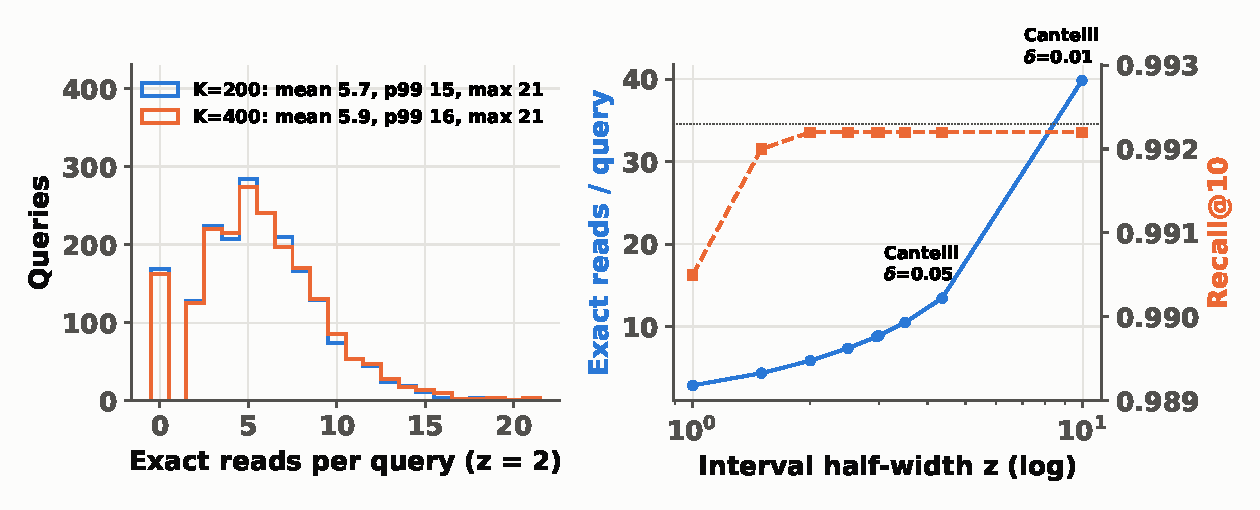
\includegraphics[width=\textwidth]{figs/fig_errorbars.pdf}
\caption{Left: distribution of exact reads per query at $z=2$ ($n_p=32$; 2{,}000 queries). A query never needs exactly one read, because a single ambiguous candidate would be decided by its neighbours' bounds. Right: reads and recall versus the interval half-width at $K=400$; the dotted line is the candidate-set ceiling.}
\label{fig:eb}
\end{figure}

\paragraph{Read-count distribution.} At $z=2$ the reads per query have median 5--6, p99 15--16 and maximum 21--22 for both $K=200$ and $K=400$, and 8\% of queries need no read at all (Figure~\ref{fig:eb}). The number of reads tracks the difficulty of the query: its Spearman correlation with the true gap between the 10th and 11th scores is $-0.54$ to $-0.56$. With $k=100$ the error bars still find the candidate ceiling exactly, with 54--56 reads per query (p99: 94--98), i.e.\ 2.7--5.4\% of the candidates (Table~\ref{tab:k100}).

\paragraph{Error bars with the tiered code.} The measurements above use FanarVSE-v1. With the final engine ($K=400$, $n_p=384$ and 768) the standardised error, with the engine's conservative $\sigma$, has mean $-0.001$ and standard deviation 0.912 over the 800{,}000 query--candidate pairs. At $z=2$ the error bars again reach the candidate-set ceiling (0.9919 against 0.9921 and 0.9959 against 0.9960) with 6.6 reads per query (p99 17, maximum 25). The certified setting of Corollary~\ref{cor:tier}, $z=4.9$ for a per-query bound $2K e^{-z^2/2}$ of 0.49\%, costs 18.1 reads (p99 43) and 7\% of throughput (21{,}057 against 22{,}719 QPS at $n_p=384$); no query had an uncovered candidate there, and 0.1\% at $z=4.36$. An exact rerank of all 400 candidates, also by zero-copy, gives the same recall at 6{,}039 QPS.

\paragraph{Seeds.} Over five seeds for every random choice (rotations, tiered rotations, coarse quantizers), recall@10 of the final engine varied by at most 0.0013 at each operating point, throughput by under 1\% and reads by at most 0.10 per query (Supplementary Note~\ref{sn:seeds}).

\subsection{Direct tests of the theory}\label{sec:tests}
The measurements above test the theory through its consequences for search; Supplementary Note~\ref{sn:tests} tests each statement directly, and Figure~\ref{fig:theory} summarises the results. (i) The exact law of Corollary~\ref{cor:law} holds down to eight dimensions, where it and a Gaussian differ: at $D=8$, 3.03\% of the errors exceed $2\sigma$ (law 3.00\%, Gaussian 4.55\%) and none exceeds $3\sigma$, because the law's support ends at $\sqrt7\approx2.65$ (Supplementary Table~\ref{tab:law}). (ii) For a fixed query--vector pair under 1{,}000 Haar rotations, the per-pair mean and spread of $Z$ agree with Theorem~\ref{thm:main} in 10 of 11 settings; the exception disappears in double precision. (iii) $Z$ is uncorrelated with the true score and with $c$, and its spread does not depend on whether a candidate is a true neighbour. (iv) Lemma~\ref{lem:cov} held in all 19{,}803 query runs whose intervals covered every candidate, and the block-max selection returned the exact top-$K$ up to fp16 ties. (v) With the engine's interval the union bound holds with a margin of 3--6$\times$; with the exact $\sigma$ the observed failure shares lie slightly above it, within sampling error. (vi) Under synthetic unbiased errors of controlled covariance, recall is a function of $\mathrm{tr}(\Sigma_qE)$ ($R^2=0.998$), not of the MSE ($R^2=0.20$), which isolates the error-isotropy principle of Section~\ref{sec:isotropy}. (vii) Out of sample, on GloVe-100 and for $k=1$ to 100, the identification estimate lies between the bits needed with 200 and with 2{,}000 candidates, but it ignores the candidate budget and does not rank the datasets reliably (Supplementary Table~\ref{tab:ident2}).

\begin{figure}[!htbp]
\centering
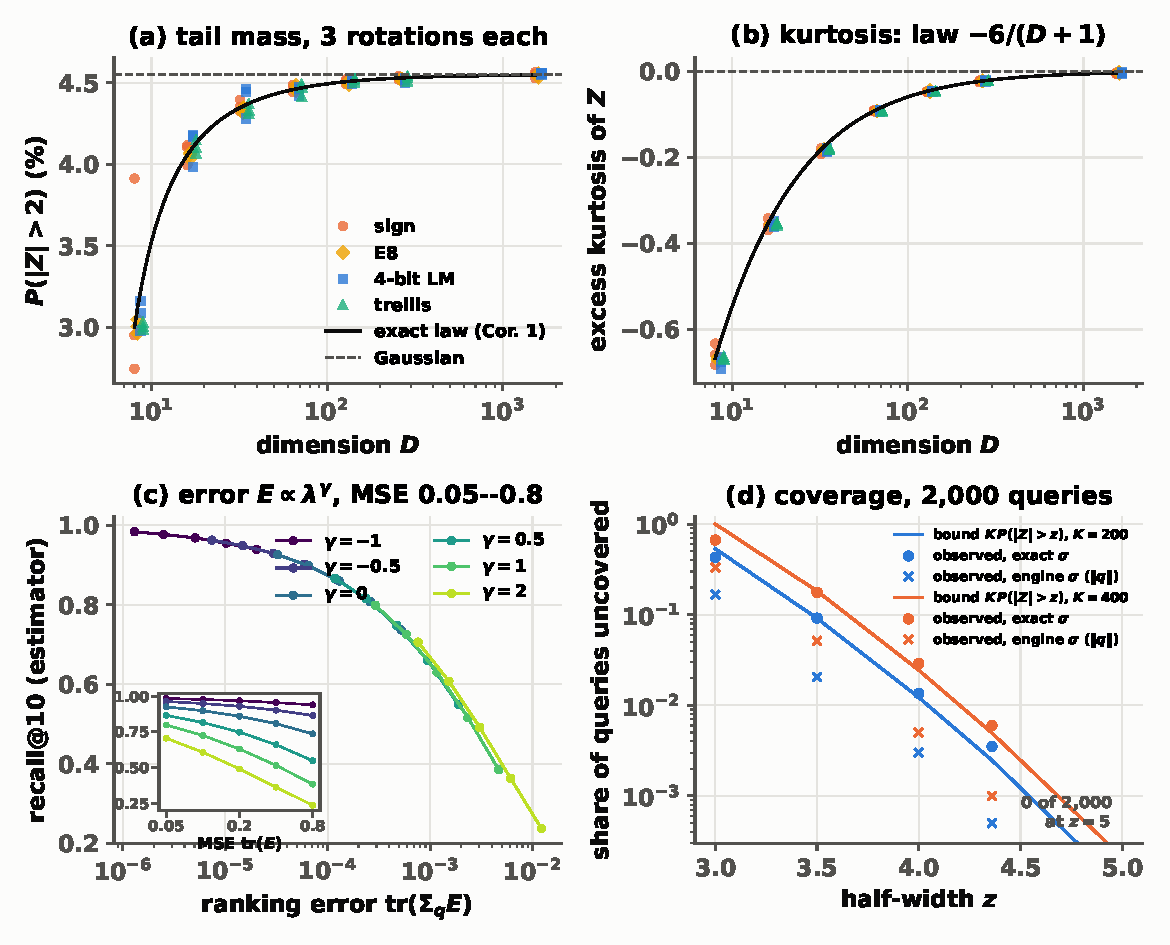
\includegraphics[width=\textwidth]{figs/fig_theory.pdf}
\caption{Direct tests of the theory. (a, b) Tail mass and excess kurtosis of the standardised error $Z$ against the dimension, on OpenAI vectors projected to $D$ principal dimensions; the solid lines are the exact law of Corollary~\ref{cor:law}, the dashed lines a Gaussian. (c) Recall of the estimator under synthetic unbiased errors with covariance $\propto\lambda^\gamma$ and MSE 0.05--0.8: recall falls on one curve in the ranking error $\mathrm{tr}(\Sigma_qE)$, not in the MSE (inset). (d) Share of queries with at least one candidate outside its interval, against the union bound $K\,P(|Z|>z)$, with the exact $\sigma$ and with the engine's conservative $\sigma$.}
\label{fig:theory}
\end{figure}


\subsection{\texorpdfstring{Larger $k$ and smaller batches}{Larger k and smaller batches}}
\paragraph{$k=100$.} Table~\ref{tab:k100} reports recall@100. FanarVSE needs $K=1{,}000$--$3{,}000$ candidates. Its threshold selection does not rescore, so its cost grows only slowly with $K$: FanarVSE reaches 0.986 at 11{,}247 QPS, 0.994 at 8{,}260 (2.5$\times$ CAGRA at 0.990), 0.997 at 6{,}507 (3.8$\times$ CAGRA at 0.996 and 11.9$\times$ IVF-RaBitQ at 0.995) and 0.999 at 4{,}374, 2.8$\times$ fp16 brute force, which is exact. The error bars reach the candidate-set ceiling in every row with 63--64 reads per query, 2--6\% of the candidates; stage 1's candidate ceiling, not the error bars, limits recall.

\begin{table}[!htbp]
\caption{Recall@100 at 998k vectors (batch 500, mean of three runs; FanarVSE with 4{,}096 cells and $R=256$). For FanarVSE, the error bars reach the candidate-set ceiling in every row.}
\label{tab:k100}
\small
\begin{tabular}{lrrrr}
\toprule
Engine & GPU B/vec & Recall@100 & QPS & Reads/query \\
\midrule
FAISS-GPU flat fp16 & 3{,}072 & 1.000 & 1{,}568 & -- \\
CAGRA deg32, itopk 256 & 3{,}200 & 0.975 & 6{,}940 & -- \\
CAGRA deg32, itopk 512, MC & 3{,}200 & 0.990 & 3{,}361 & -- \\
CAGRA deg32, itopk 1024 & 3{,}200 & 0.996 & 1{,}734 & -- \\
CAGRA deg64, itopk 1024 & 3{,}328 & 0.997 & 891 & -- \\
IVF-RaBitQ 9 bit, 4{,}096 lists, $n_p$=384 & 1{,}851 & 0.988 & 1{,}068 & -- \\
IVF-RaBitQ 9 bit, 4{,}096 lists, $n_p$=768 & 1{,}851 & 0.995 & 548 & -- \\
FanarVSE $n_p$=512, $K$=1{,}000 & 570 & 0.986 & 11{,}247 & 63 \\
FanarVSE $n_p$=1{,}024, $K$=1{,}500 & 570 & 0.994 & 8{,}260 & 64 \\
FanarVSE $n_p$=1{,}536, $K$=2{,}000 & 570 & 0.997 & 6{,}507 & 64 \\
FanarVSE $n_p$=3{,}072, $K$=3{,}000 & 570 & 0.999 & 4{,}374 & 64 \\
\bottomrule
\end{tabular}
\end{table}

\paragraph{Batch size and latency.} Table~\ref{tab:lat} measures each engine one batch at a time, so the time per batch is the latency a client sees when that many requests are served together (a closed loop with that many concurrent clients and dynamic batching). With the small-batch path (Section~\ref{sec:system}) a single query takes 0.84--1.16\,ms with the final engine: less than with IVF-RaBitQ (1.45\,ms) and 1.2--1.3$\times$ as long as with CAGRA at similar recall. At a batch of 16 FanarVSE at 0.992 takes 4.7\,ms, between IVF-RaBitQ at 0.992 (4.1\,ms) and CAGRA at 0.99 (5.7\,ms), and at 0.982 4.0\,ms against 2.9\,ms for CAGRA at 0.98--0.99. From a batch of 100 upward it is the fastest of the three: at recall 0.992 a batch of 100 takes 9.0\,ms against 15.5\,ms for IVF-RaBitQ and 30.4\,ms for CAGRA at 0.99, and a batch of 500 takes 21\,ms against 62\,ms and 148\,ms. The efficacy of the error bars does not depend on the batch size: reads per query are the same at every batch size, since each query is tested independently.

\begin{table}[!htbp]
\caption{Median time per batch (ms) when batches are served one at a time (998k vectors, $k=10$). CAGRA and IVF-RaBitQ use the RMM pool and their best search algorithm.}
\label{tab:lat}
\small
\begin{tabular}{lrrrrr}
\toprule
Engine (recall@10) & batch 1 & 16 & 100 & 500 & QPS at 500 \\
\midrule
CAGRA itopk 256 (0.98--0.99) & 0.64 & 2.9 & 13.1 & 64 & 7{,}842 \\
CAGRA itopk 512, MC (0.99) & 0.78 & 5.7 & 30.4 & 148 & 3{,}368 \\
IVF-RaBitQ 9 bit, $n_p$=384 (0.992) & 1.45 & 4.1 & 15.5 & 62 & 8{,}079 \\
FanarVSE $n_p$=256, $K$=200 (0.982) & 0.84 & 4.0 & 7.4 & 16 & 28{,}684 \\
FanarVSE $n_p$=384, $K$=400 (0.992) & 0.95 & 4.7 & 9.0 & 21 & 22{,}649 \\
FanarVSE $n_p$=768, $K$=400 (0.996) & 1.16 & 5.1 & 9.3 & 25 & 19{,}624 \\
\bottomrule
\end{tabular}
\end{table}

\subsection{Throughput mode at large batches}\label{sec:tput}
CAGRA's throughput does not grow with the batch: at itopk 384 it serves 4{,}430, 4{,}459 and 4{,}480 QPS at batches of 500, 2{,}000 and 4{,}000 (recall 0.990--0.991), because each query walks the graph on its own. FanarVSE shares each code block among all the queries that probe its cell, so larger batches amortise its scan and its fixed costs. Table~\ref{tab:tput} measures FanarVSE-T (Section~\ref{sec:tmode}) at batches of 500 to 16{,}000. We hold only 2{,}000 queries with ground truth, so batches of 4{,}000 and 16{,}000 repeat them two and eight times, for CAGRA as well; at a batch of 2{,}000, repeating each of 1{,}000 queries twice raised FanarVSE-T's throughput by less than 1\% (and four times, by at most 3.4\%), so the repetition barely helps it.

At a batch of 2{,}000, every query distinct, FanarVSE-T reaches recall 0.9905 at 83{,}606 QPS, 18.8$\times$ CAGRA at 0.9904, and 0.9931 at 71{,}605, 21$\times$ CAGRA at 0.993. At a batch of 16{,}000 (about 180\,ms per batch) it reaches 0.9905 at 90{,}391 QPS (20$\times$ CAGRA), 0.996 at 54{,}664 (24$\times$) and 0.9969 at 46{,}622 (27$\times$); with $z=1.5$ and every candidate scored it reaches 0.998 at 39{,}316 QPS at a batch of 4{,}000, 44$\times$ the throughput of CAGRA at its highest recall (0.9975 at 892 QPS), and 0.9994 at 23{,}905. Against the default engine, FanarVSE-T is 2.7$\times$ faster near recall 0.992 at a batch of 500 (60{,}030 against 22{,}649 QPS) and 2.6$\times$ at a batch of 2{,}000, with 1.4$\times$ its memory. The error bars cost 4.2 exact reads per query at every operating point. Queries that fail the count check (0--2.6\% up to recall 0.997, about half at $n_p\ge1{,}536$, where the buffers should grow) are recomputed, so every result is the exact top $K$ of the estimates. At a batch of 500 the $n_p=768$ point is slower than $n_p=1{,}024$ (32{,}214 against 33{,}682 QPS), although both recompute 2\% of the queries; we did not find the cause.

\begin{table}[!htbp]
\caption{Throughput mode (FanarVSE-T, 787\,B/vector) against CAGRA (3{,}200\,B/vector) and the default engine (570\,B/vector) by batch size (998k OpenAI vectors, $k=10$, FanarVSE-T with $z=1.25$ unless stated, best of three timed runs, default engine at batch 500 mean of three; batches of 4{,}000 and 16{,}000 repeat the 2{,}000 queries). Recall and reads per query do not depend on the batch. CAGRA rows give recall at batch 4{,}000 (0.9904--0.9930 at the smaller batches). ``--'': not measured.}
\label{tab:tput}
\small
\setlength{\tabcolsep}{4pt}
\begin{tabular}{lrrrrrr}
\toprule
Engine & Recall@10 & Reads & \multicolumn{4}{c}{QPS at batch} \\
 & & /query & 500 & 2{,}000 & 4{,}000 & 16{,}000 \\
\midrule
CAGRA deg32, itopk 384, MC & 0.991 & -- & 4{,}430 & 4{,}459 & 4{,}480 & -- \\
CAGRA deg32, itopk 512, MC & 0.993 & -- & 3{,}368 & 3{,}390 & 3{,}397 & -- \\
CAGRA deg32, itopk 768, MC & 0.996 & -- & -- & -- & 2{,}301 & -- \\
CAGRA deg32, itopk 1024, MC & 0.997 & -- & -- & -- & 1{,}739 & -- \\
CAGRA deg64, itopk 1024, MC & 0.9975 & -- & -- & -- & 892 & -- \\
FanarVSE (default), $n_p$=384, $K$=400 & 0.992 & 6.6 & 22{,}649 & 30{,}600 & -- & -- \\
\midrule
FanarVSE-T $n_p$=256, $K$=150 & 0.9857 & 4.2 & 48{,}107 & 80{,}544 & 89{,}216 & 101{,}410 \\
FanarVSE-T $n_p$=320, $K$=175 & 0.9893 & 4.2 & 61{,}810 & 86{,}532 & 89{,}118 & 93{,}693 \\
FanarVSE-T $n_p$=352, $K$=175 & 0.9905 & 4.2 & 60{,}994 & 83{,}606 & 86{,}215 & 90{,}391 \\
FanarVSE-T $n_p$=384, $K$=175 & 0.9916 & 4.2 & 60{,}030 & 80{,}684 & 83{,}353 & 87{,}404 \\
FanarVSE-T $n_p$=448, $K$=250 & 0.9931 & 4.2 & 54{,}648 & 71{,}605 & 73{,}696 & 76{,}434 \\
FanarVSE-T $n_p$=512, $K$=300 & 0.9940 & 4.2 & 51{,}890 & 66{,}980 & 68{,}229 & 70{,}263 \\
FanarVSE-T $n_p$=768, $K$=400 & 0.9960 & 4.2 & 32{,}214 & 50{,}881 & 52{,}062 & 54{,}664 \\
FanarVSE-T $n_p$=1024, $K$=400 & 0.9969 & 4.2 & 33{,}682 & 44{,}097 & 45{,}421 & 46{,}622 \\
FanarVSE-T $n_p$=1024, $K$=400, $z$=1.5, no $\delta$\textsuperscript{*} & 0.9980 & 5.1 & -- & -- & 39{,}316 & -- \\
FanarVSE-T $n_p$=2048, $K$=600, $z$=1.5, no $\delta$\textsuperscript{*} & 0.9994 & 5.1 & -- & -- & 23{,}905 & -- \\
\bottomrule
\end{tabular}

{\footnotesize \textsuperscript{*}Measured before the routing and tile changes of Section~\ref{sec:tmode} (unnormalised table of cell means, $r=0.75K$, larger emit tiles); with $z=1.25$ and the $\delta$ rule recall stops at 0.9978.}
\end{table}

\subsection{Three more operating points}\label{sec:points}
\paragraph{Single queries.} For one query the time is in fixed costs, not in the scan: of 0.99\,ms, 0.78\,ms were GPU work and the rest host overhead, and inside the GPU work the routing product with the cell means was computed twice (once for routing, once for the stage-1 constants), the first pass's block maxima were selected over all 31k blocks of the index, and the emit buffer was sorted at its full width. A dedicated path for one query routes and builds the constants from one product, keeps the first-pass maxima only for the blocks of the first-pass cells, and copies the ids and the exactness flag into pinned host memory inside the CUDA graph, so that a search is one graph replay and one stream synchronisation. With the cell means projected on the stage-1 basis (2\,MB instead of 12.6\,MB; recall 0.0004--0.0025 lower), a single query takes 0.54\,ms at recall 0.981 and 0.63\,ms at 0.991, against 0.64\,ms and 0.78\,ms for CAGRA at 0.98--0.99 and 0.99; with the exact means, 0.69\,ms at 0.992. Queries that fail the count check (1--2\%) are recomputed on the general path, which sets the 99th percentile at 1.3--1.9\,ms.

\paragraph{Under eight bytes of GPU memory per vector.} Each batch reads every stage-1 code block once, so stage 1 can read its codes from pinned host memory over PCIe almost as fast as from device memory: with the stage-1 codes and scales in host RAM, throughput falls by 3\%. Moving every per-vector array to host RAM (stage-1 codes, refinement records, full vectors stored in cell order so that no id map is needed on the GPU, and the id map itself) leaves only shared tables on the GPU; with the cell means projected on the stage-1 basis and the query-side matrices in fp16 (recall and reads unchanged), they take 7.7\,MB for 998k vectors, under 8\,B per vector and falling with $N$. Every candidate's refinement record then crosses PCIe, which makes stage 2 the bottleneck (29\,ms of 44\,ms per batch at $K=400$), so smaller records pay: with 2{,}048 refinement bits (280-byte records, 28.5 exact reads per query) the engine reaches 0.991 at 13{,}841 QPS, 0.995 at 12{,}587 and 0.998 at 7{,}912 (9{,}214 with 1{,}536 bits). At 0.991 this is 3.1$\times$ the throughput of CAGRA and 1.7--1.9$\times$ that of IVF-RaBitQ at 0.992, with 415$\times$ and 240$\times$ less GPU memory; host RAM holds 3.4\,KB per vector, of which 3{,}072\,B are the fp16 vectors.

\paragraph{A graph front-end for throughput.} At recall 0.99 the cell scan scores about 94k codes per query, so we also built an optional graph mode that replaces only stage 1: a beam search, written in CUDA, over a pruned 32-neighbour graph (Vamana rule with $\alpha=1$~\cite{subramanya2019diskann}) with 256-byte int8 navigation codes, which hands its best 128 candidates to stages 2 and 3 (Supplementary Note~\ref{sn:graph}). It scores 14$\times$ fewer codes per query, but each step is a dependent random read, and on this GPU the walk saturates at about $2.5\times10^8$ scores per second. End to end it is 1.2--1.3$\times$ faster than the default near recall 0.99 and on par above it, with 904 instead of 570\,B/vector and no exact stage-1 selection (Table~\ref{tab:graph}). It is an option where throughput near recall 0.99 matters more than memory.

\begin{table}[!htbp]
\caption{Graph front-end against the default stage 1 (998k OpenAI vectors, $k=10$, batch 500, best of three runs). Both share stages 2 and 3. Ceiling: recall of the candidate set handed to stage 2. $L$: beam width.}
\label{tab:graph}
\small
\begin{tabular}{lrrrrr}
\toprule
Stage 1 & GPU B/vec & Scores/query & Ceiling & Recall@10 & QPS \\
\midrule
Cell scan, $n_p$=384, $K$=400 (default) & 570 & $\approx$94k & -- & 0.992 & 22{,}649 \\
Graph, $L$=256, $K$=128 & 904 & 4{,}385 & 0.9894 & 0.9882 & 25{,}620 \\
Graph, $L$=384, $K$=128 & 904 & 6{,}596 & 0.9916 & 0.9905 & 28{,}770 \\
Graph, $L$=512, $K$=128 & 904 & 8{,}912 & 0.9938 & 0.9926 & 23{,}336 \\
\bottomrule
\end{tabular}
\end{table}

\subsection{Scaling beyond one million vectors}
With 16\,GB of host RAM we cannot hold a 10M-vector set of 1536-dimensional embeddings (31\,GB in fp16) together with the lean variant's 5\,GB of refinement records, so we measured the part of FanarVSE whose cost grows with $N$. Replicating the stage-1 codes up to 10M vectors, a full stage-1 scan for 500 queries takes 85, 144, 328 and 633\,ms at 1M, 2M, 5M and 10M vectors (362\,MB of stage-1 codes at 10M), i.e.\ it grows linearly; with routing the work is proportional to $N n_p/n_{\mathrm{cells}}$. Stages 2 and 3 depend on $K$ and the number of reads, not on $N$. To measure the whole engine (the intermediate engine of Table~\ref{tab:chain}), we replicated the 1M index two and four times inside each cell (codes, factors and refinement planes), so that the same probes scan two and four times as many vectors: at $n_p=768$, $K=400$ throughput falls from 17.0k to 11.5k and 7.5k QPS (2.2\,GB of GPU memory at 4M), i.e.\ 4$\times$ the scanned data costs 2.3$\times$ the time, because the fixed per-batch costs are amortised. At 10M the final engine would need 5.5\,GB of GPU memory, the lean variant 0.45\,GB and the host-resident mode of Section~\ref{sec:points} a few tens of megabytes for its tables. Encoding is linear too, about 21\,s per 10M vectors (Section~\ref{sec:trellis}). Recall at 10M--100M depends on the data and remains untested.

\subsection{Image embeddings and larger collections}\label{sec:more}
To test the method beyond one embedding family, we ran the final engine unchanged (refinement of 2.5 bits per dimension, $z=2$) on five more sets, each with 2{,}000 held-out queries and exact inner-product ground truth: OpenAI text-embedding-3-large vectors (98k, 1536 dimensions) and arXiv InstructorXL title embeddings (98k, 768 dimensions); the full arXiv InstructorXL set (2.25M vectors); SigLIP image embeddings of the ImageNet-1k training images (1.28M, 768 dimensions); and DINOv2-giant image embeddings of the Metropolitan Museum's open-access collection (258k, 1536 dimensions). We use 512 cells for the 98k sets, 1{,}024 for DINOv2, 4{,}096 for SigLIP and 8{,}192 for the 2.25M set, and $R=256$ except for DINOv2, whose flatter spectrum needs $R=512$ ($R=768$ exceeds the shared memory of our stage-1 kernels). The baselines follow the protocol of Section~\ref{sec:eval}: an RMM pool, CAGRA over itopk 32 to 1{,}024, degrees 32 and 64 and all four search algorithms, and IVF-RaBitQ over 4 to 9 bits and all probe counts. Table~\ref{tab:other} gives the fastest configuration of each engine at four recall targets. On every set the error bars reach the candidate-set ceiling to within 0.0005.

\paragraph{Text embeddings.} FanarVSE is the fastest index at every target on both 98k sets (2.4--14$\times$ CAGRA and 2.2--5.5$\times$ IVF-RaBitQ), and on the 2.25M arXiv set from recall 0.98 upward (1.3--3.8$\times$ CAGRA, 1.8--3.0$\times$ IVF-RaBitQ); there it is also 2.3$\times$ faster than fp16 brute force at the recall of brute force. At 0.95--0.97 CAGRA is faster on the 2.25M set (25{,}150 against 12{,}290 QPS at 0.95). At 98k, brute force is a strong baseline: FanarVSE passes it on the 1536-dimensional OpenAI set (52{,}695 QPS at 0.993 against 43{,}561 at 0.998) but not on the 768-dimensional arXiv set, where brute force (67{,}657 QPS at 0.993) is faster than every index.

\paragraph{Image embeddings.} On both image sets IVF-RaBitQ with 9 bits per dimension is faster than FanarVSE at moderate recall: by 1.25--1.35$\times$ up to 0.99 on DINOv2 and by 1.2--1.6$\times$ up to 0.995 on SigLIP, with 3.4$\times$ and 3.1$\times$ more GPU memory. Its estimator ranks these vectors well enough to need no exact reads, and it saturates at 0.993 and 0.9965. FanarVSE is the fastest index above those points (3.3$\times$ CAGRA at 0.995 on DINOv2 and 2.5$\times$ at 0.998 on SigLIP) and is 1.8$\times$ and 5.6$\times$ faster than fp16 brute force at its recall. On SigLIP FanarVSE does not exceed about 28k QPS even at low recall: with 500 queries nearly every cell is probed by some query, so stage 1 decodes almost the whole index twice per batch (first pass and emit), and IVF-RaBitQ's scan is cheaper per vector. The 768-dimensional refinement code has half the bits of the 1536-dimensional one, so exact reads rise from 8 per query on the OpenAI sets to 15--18 on the arXiv sets and 26--30 on SigLIP (16--20 on DINOv2); coding stage 2 from the cell mean cuts SigLIP's to 16.5 (Section~\ref{sec:system}).

\paragraph{The cell-residual stage 1 across datasets.} Against the global-centre stage 1 of the intermediate engine, measured at matched recall with the same refinement code, the cell residual raised throughput by 1.0--1.5$\times$ on the text sets, 1.25--1.7$\times$ on SigLIP and 1.6--2.3$\times$ on DINOv2, where the global-centre code needed $K=800$ candidates for recall 0.99 and the cell-residual code 200. The gain is largest where the data are most clustered.

\begin{table}[!htbp]
\caption{Five more datasets: QPS (and recall@10) of each engine's fastest configuration that reaches the target recall (2{,}000 queries, $k=10$, batch 500, mean of three runs; ``--'': target not reached). GPU memory per vector: FanarVSE including its shared tables; IVF-RaBitQ measured as the drop in free device memory (including fixed overheads, which weigh more at 98k).}
\label{tab:other}
\small
\setlength{\tabcolsep}{11pt}
\begin{tabular}{lrrrr}
\toprule
Dataset & Target & FanarVSE & CAGRA & IVF-RaBitQ (9 bit) \\
\midrule
\multicolumn{5}{@{}l@{}}{\parbox{12.6cm}{\emph{OpenAI-3-large, 98k $\times$ 1536 (B/vec: FanarVSE 670, CAGRA 3{,}200--3{,}328, IVF-RaBitQ 2{,}461); fp16 brute force 43{,}561 QPS at 0.998}}} \\
 & 0.98 & 63{,}012 (0.982) & 14{,}077 (0.988) & 20{,}594 (0.985) \\
 & 0.99 & 52{,}695 (0.993) & 7{,}645 (0.994) & 12{,}909 (0.995) \\
 & 0.995 & 43{,}728 (0.996) & 4{,}606 (0.996) & 7{,}905 (0.998) \\
 & 0.998 & 34{,}288 (0.999) & 2{,}406 (0.999) & 7{,}905 (0.998) \\
\multicolumn{5}{@{}l@{}}{\parbox{12.6cm}{\emph{arXiv InstructorXL, 98k $\times$ 768 (B/vec: 342, 1{,}664--1{,}792, 1{,}455); fp16 brute force 67{,}657 QPS at 0.993}}} \\
 & 0.98 & 60{,}490 (0.984) & 25{,}136 (0.982) & 21{,}024 (0.990) \\
 & 0.99 & 46{,}886 (0.992) & 12{,}973 (0.994) & 21{,}024 (0.990) \\
 & 0.995 & 38{,}757 (0.997) & 8{,}510 (0.997) & 13{,}214 (0.997) \\
 & 0.998 & 28{,}075 (0.999) & 6{,}519 (0.998) & -- \\
\multicolumn{5}{@{}l@{}}{\parbox{12.6cm}{\emph{arXiv InstructorXL, 2.25M $\times$ 768 (B/vec: 309, 1{,}664--1{,}792, 925); fp16 brute force 3{,}010 QPS at 0.993}}} \\
 & 0.95 & 12{,}290 (0.968) & 25{,}150 (0.951) & 8{,}862 (0.964)$^\dagger$ \\
 & 0.98 & 10{,}378 (0.983) & 8{,}043 (0.985) & 5{,}945 (0.980) \\
 & 0.99 & 7{,}636 (0.990) & 4{,}163 (0.992) & 3{,}671 (0.990) \\
 & 0.995 & 6{,}107 (0.995) & 1{,}616 (0.998) & 2{,}024 (0.996) \\
\multicolumn{5}{@{}l@{}}{\parbox{12.6cm}{\emph{SigLIP (ImageNet-1k images), 1.28M $\times$ 768 (B/vec: 309, 1{,}664--1{,}792, 943); fp16 brute force 4{,}452 QPS at 0.993}}} \\
 & 0.98 & 28{,}183 (0.987) & 25{,}793 (0.987) & 44{,}253 (0.989) \\
 & 0.99 & 26{,}826 (0.992) & 16{,}737 (0.990) & 36{,}587 (0.993) \\
 & 0.995 & 22{,}078 (0.995) & 13{,}671 (0.997) & 27{,}314 (0.995) \\
 & 0.998 & 19{,}552 (0.998) & 7{,}986 (0.998) & -- \\
\multicolumn{5}{@{}l@{}}{\parbox{12.6cm}{\emph{DINOv2-giant (Met images), 258k $\times$ 1536 (B/vec: 639, 3{,}200--3{,}328, 2{,}044); fp16 brute force 12{,}548 QPS at 0.990}}} \\
 & 0.98 & 26{,}843 (0.988) & 29{,}750 (0.985) & 35{,}968 (0.984) \\
 & 0.99 & 22{,}823 (0.990) & 17{,}781 (0.990) & 28{,}433 (0.990) \\
 & 0.993 & 17{,}804 (0.994) & 15{,}572 (0.993) & -- \\
 & 0.995 & 16{,}558 (0.995) & 5{,}102 (0.995) & -- \\
\bottomrule
\end{tabular}

{\footnotesize $^\dagger$5 bits per dimension (542\,B/vector).}
\end{table}

\subsection{Smaller and lower-dimensional data}
On a 229k subset of the OpenAI vectors a stage-1-only configuration reaches recall 0.999 at 13{,}584 QPS with 98\,B/vector, 14$\times$ the throughput of CAGRA, and on GloVe-100, where CAGRA and IVF-RaBitQ stay below 0.98, FanarVSE with 52\,B/vector reaches 0.999 at 20{,}544 QPS, 2.3$\times$ the throughput of exact search (Supplementary Note~\ref{sn:small}, which also gives CPU reference points).

\section{What Did Not Work}\label{sec:negative}
Table~\ref{tab:neg} lists ideas we implemented and measured that did not help, with the reason; engineering variants of the kernels that did not help are in Supplementary Table~\ref{tab:neg2}. We report them because several are natural ideas that others may try.

\begin{table}[!htbp]
\caption{Negative results (OpenAI-1536 unless noted).}
\label{tab:neg}
\small
\begin{tabular}{p{4.5cm}p{11cm}}
\toprule
Idea & Outcome \\
\midrule
Bussgang LMMSE decoding & MSE halved, recall 0.828$\to$0.793 (\S\ref{sec:isotropy}). \\
Dual-tree pruning (Barnes--Hut) & 0\% of query-cluster/cell pairs prunable; cells span about 70$^\circ$ in 1536 dims. \\
Extreme-value adaptive stopping & Needs more probes than fixed $n_p$ for equal recall. \\
kNN-graph min-cut partitioning & Cuts graph edges by a third (26\%$\to$17\%) but leaves routing recall unchanged (0.972 vs.\ 0.972 at $n_p$=8). \\
Permutation codes & Gaussian MSE 0.338 at 1 bit (trellis: 0.264). \\
Error-bar cascade in stage 1 & Correct, but prunes under 20\% of candidates; no speed gain. \\
Reduced-precision SSD reads & NVMe cost is per request (82k--88k IOPS from 512\,B to 8\,KB). \\
Neighbour co-location on SSD & Pages touched per query 10$\to$7.9 only. \\
Spilling to a second cell & With 4{,}096 cells, assigning all or the 10--40\% most ambiguous vectors also to their second-nearest (or a SOAR-like) cell covers no more of the true top-10 at equal scan cost. \\
Exact cell pruning in stage 1 & A Cauchy--Schwarz bound $\langle q,m_c\rangle+\|Wq\|\max_{x\in c}\|\hat r_x\|$ on every estimate in a probed cell never fell below the $K$-th estimate (0\% of probed cells pruned, OpenAI and SigLIP). \\
Routing by mean plus cell radius & Ranking cells by $\langle q,m_c\rangle+\kappa\|q\|r_c$ instead of the centroid direction changed candidate recall by at most 0.001. \\
Stage 2 from the cell mean & Exact reads $-20$\% (OpenAI) to $-43$\% (SigLIP), but equal or 5\% lower GPU throughput (an fp32 constant per candidate). \\
\bottomrule
\end{tabular}
\end{table}

\section{Limitations}\label{sec:limits}
\paragraph{Scope.} All measurements come from one laptop GPU (RTX 3050, 6\,GB), one NVMe drive and at most 2.25 million real vectors; behaviour on data-centre GPUs, with several GPUs and at 10M--100M vectors is untested beyond the linear cost model of stage 1. We evaluated six embedding sets for the full system (four text models, GloVe and two image models, SigLIP and DINOv2, but no jointly trained multimodal retrieval set), four for the codebook study, and two of the extra sets at only 98k vectors. We could not run Lychee, for which no implementation was available, and we did not compare with FaTRQ on shared hardware. We evaluated inner-product search only; the L2 reduction of Section~\ref{sec:modes} is untested. This study used the hardware available to us, one laptop GPU; the next phase of this work will repeat the evaluation on data-centre and multi-GPU systems and on larger and more varied datasets, including 10M--100M-vector collections and multimodal retrieval embeddings.

\paragraph{Where FanarVSE loses.} With the single-query path FanarVSE's median latency is below CAGRA's, but its 99th percentile (1.3--1.9\,ms) is set by the 1--2\% of queries that fail the count check and are recomputed; at a batch of 16 FanarVSE is up to 1.4$\times$ slower than CAGRA and 1.1$\times$ slower than IVF-RaBitQ. The host-resident mode halves throughput relative to the GPU-resident engine: its stage 2 fetches every candidate's record over PCIe. On image embeddings 9-bit IVF-RaBitQ is 1.2--1.6$\times$ faster up to recall 0.99--0.995, with three times FanarVSE's memory, and on the 2.25M arXiv set CAGRA is faster below 0.98; at 98k vectors and 768 dimensions fp16 brute force beats every index. FanarVSE's stage 1 decodes most of the index twice per large batch, which bounds its throughput at low recall (about 28k QPS on SigLIP). Stage 1 with $R=768$ exceeds the shared memory of our kernels. We did not compare the engines below recall 0.945. The current engine's selection kernels were tuned on one GPU and one dataset (4{,}096 cells, batch 500); the speed-ups of Table~\ref{tab:chain} may differ on other hardware. The throughput mode needs large batches: its 19--27$\times$ lead over CAGRA holds at batches of 2{,}000 to 16{,}000 (tens to 180\,ms per batch), falls to 14$\times$ at a batch of 500 near recall 0.99, and was measured on one dataset only; it uses 1.4$\times$ the GPU memory of the default, its $\delta$ rule has no guarantee, and with $z=1.25$ it gives up 0.0003 of recall. The optional graph front-end (Section~\ref{sec:points}) gains only 1.2--1.3$\times$ near recall 0.99 for 1.6$\times$ the GPU memory, because on this GPU its random reads cost as much per query as the ordered cell scan.

\paragraph{Guarantees.} Corollary~\ref{cor:law} and the coverage bound hold for a Haar rotation and are in probability over the random rotation, not for every fixed index; for structured rotations we have only the measurements of Table~\ref{tab:rot}. The default $z=2$ is not certified; the certified setting costs 13 reads per query (18 with the tiered code, whose certificate uses the looser sub-Gaussian bound of Corollary~\ref{cor:tier}). With the exact $\sigma$, the share of queries with an uncovered candidate lay slightly above the union bound on our index (within sampling error); the engine's conservative interval stays 3--6$\times$ below it. The direct tests of Section~\ref{sec:tests} use one embedding family (OpenAI) for the law and up to 1{,}000 rotations per pair, which detects departures of a few hundredths of $\sigma$ but not smaller ones. The identification-rate estimate assumes i.i.d.\ Gaussian coordinates, depends strongly on the definition of the effective dimension and ignores the candidate budget; out of sample it is right only to within a factor of two, and we use it as a guide only; an extension that models the candidate budget through the order statistics of the similarities is open. We have no analytical bound for structured rotations, and the tiered code's certificate uses a sub-Gaussian bound that is looser than the exact law of a single tier. Table~\ref{tab:modes} states which of these applies in each mode.

\paragraph{Engineering.} The lean variant moves 512\,B/vector of refinement records to host RAM rather than eliminating them, and full vectors still occupy RAM or NVMe; it needs the GPU to read pinned host memory directly. The query path is Python with Triton kernels inside CUDA graphs; a single query spends 0.78\,ms of its 1.0\,ms in GPU work, most of it in fixed per-call costs (buffer initialisation, selection over all blocks, some 40 small kernels).

\section{Conclusion}
Coding theory supplies three tools that a GPU vector index can use directly: an exact error law that holds for any rotated codebook, trellis codes that sit within a fraction of a decibel of the Shannon bound, and an identification rate that suggests how small a filter can be. Combined with error bars that limit full-precision reads to about six per query, or to 13--18 with a per-query guarantee, an exact threshold selection, a first stage coded from the cell means and a tiered refinement code, they let one laptop GPU search a million 1536-dimensional vectors at recall 0.992 at 22{,}600 queries per second with 570 bytes of device memory per vector, or at 13{,}800 queries per second with under eight bytes per vector when every per-vector array stays in host RAM, faster than CAGRA and IVF-RaBitQ at every recall we measured from 0.95 upward with a third or less of their memory, up to the recall of exact search, and with a single-query latency of about a millisecond. For large batches, int8 first-stage codes and a refinement code scored by lookup tables raise this to 83{,}600--90{,}400 queries per second at recall 0.99 with 787 bytes per vector, 19--20$\times$ CAGRA on the same GPU. The same engine, unchanged, is the fastest index at high recall on image embeddings and on 2.25 million arXiv vectors, but IVF-RaBitQ on image embeddings and CAGRA on the largest set are faster at moderate recall, and graphs remain faster for small batches. The main open items are a first stage that does not decode most of the index twice per batch, a faster path for batches of 2--32 queries, and evaluation on more GPUs, at larger scale and on multimodal retrieval embeddings, which is the next phase of this work.

\bibliography{refs}

\section*{Data Availability}
The DBpedia OpenAI-ada-002 embeddings and the GloVe-100 dataset are publicly available, as are the extra sets of Section~\ref{sec:more}: DBpedia OpenAI text-embedding-3-large (Qdrant/dbpedia-entities-openai3-text-embedding-3-large-1536-100K), arXiv InstructorXL title embeddings (Qdrant/arxiv-titles-instructorxl-embeddings), SigLIP embeddings of ImageNet-1k (mlnomad/imagenet-1k-224-clip-embeddings) and DINOv2-giant embeddings of the Metropolitan Museum's open-access images (metmuseum/openaccess-embeddings-dinov2-giant, CC0), all on Hugging Face; query selection and ground truth are produced by our scripts. The FanarVSE source code will be released upon publication. It includes the Triton kernels (trellis decoding and scan, threshold-and-emit selection with cell-residual constants, the synchronisation-free batch path, small-batch and probe-mask selection, fused tiered refinement, zero-copy exact reads, fused Viterbi encoder, and the int8 stage-1 and lookup-table stage-2 kernels of the throughput mode), the index builder, and the scripts that produce every table and figure (including the \texttt{ctypes} binding used to call cuVS IVF-RaBitQ), together with ground-truth files and the raw result logs (JSON) for every number in this paper.

\section*{Ethics}
The work uses public, non-personal embedding datasets and involves no human subjects.

\section*{Research Funding}
This research received no external funding; it was funded personally by the author.

\section*{Author contributions}
M.M. conceived the study, designed the methods, implemented the software, ran the experiments and wrote the manuscript. The author reviewed and approved the final manuscript.

\section*{Competing interests}
The author declares no competing interests.

\section*{Additional information}
Correspondence and requests for materials should be addressed to M.M.

\end{document}
